\documentclass[12pt, a4paper]{article}
\usepackage{amsfonts, amsmath, amsthm}
\usepackage[utf8x]{inputenc}
\usepackage{indentfirst}
\usepackage{multirow}
\usepackage[table]{xcolor}
\usepackage{listings}
\usepackage{alltt}
\usepackage{fancyvrb}
\usepackage{graphicx}
\usepackage{algorithm}
\usepackage{algpseudocode}
\usepackage{subfigure}
\usepackage{setspace}
\usepackage{wrapfig}
\usepackage{colortbl}
\usepackage{wrapfig}
\usepackage{tikz}
%\usepackage{subfig}
%\usepackage[hyphens]{url}
\usepackage{setspace}
\usepackage{hyperref}

\hypersetup{
	colorlinks,
	linkcolor={red!50!black},
	citecolor={green!80!black},
	urlcolor={blue!80!black}
}


\usetikzlibrary{positioning}
\graphicspath{ {./images/} }


\title{%
	
\includegraphics[height=0.3\textwidth]{UNITBV2.png}~ 
	\\[1cm]
	\vspace{20mm}
	
	\bf 	LUCRARE DE LICENȚĂ
	\noindent\rule{14cm}{1pt}
	\bf Serenity Garden TD
}

\date{}

\begin{document}
	
	
	
	\maketitle
	\vspace{10mm} %5mm vertical space
	\begin{flushleft}
		\bf 	Conducător Științific:
		\bf     \\Lector Universitar Deaconu Adrian
	\end{flushleft}
	
	\begin{flushright}
		\bf Absolvent:
		\bf \\Opria Ion-Bogdan
	\end{flushright}
	
	\vspace{4mm} %5mm vertical space
	
	\begin{center}
		\bf Brașov, 2021 
	\end{center}
	
	
	\tableofcontents
	\pagebreak
	
	\section{Introducere}
	
	
	
	
	
	\subsection{Descrierea proiectului}
	
	Jocurile video au început să acapareze din ce în ce mai mult viețile noastre datorită ușurinței de accesare și a experienței pe care o oferă. Odată cu evoluția hardware-ului, jocurile video au devenit din ce în ce mai realiste și prin urmare oferă experiențe care nu poat fi găsite în niciun alt mediu existent, deoarece în nici un alt mediu nu putem controla și traii experiențele unor personaje atât de indetaliat. Industria jocurilor video este o industrie care este în continuă creștere și prin urmare este o ramură care merită explorată din perspectiva unui programator și nu nu mai. 
	\newline
	
	"Games are great to work on because they are as much about art as they are science." \cite{gameProgrammingComplete}
	\newline
	
	Din aceste motive, am ales drept proiect pentru licență să creez un joc video. Jocul se numește "Serenity Garden TD" și este un tower defense 3D. Experiența jocului are loc în câteva nivele special definite, în care utilizatorul trebuie să își protejeze baza de operații. Există multe tipuri diferite de inamici care vor să distrugă baza jucătorului, iar acesta, pentru a o proteja, trebuie să construiască un sistem defensiv. Jucătorul poate să construiască turnuri defensive care au diferite efecte asupra inamicilor. Inamicii atacă sistemul defensiv, sau în cazul în care lipsește, atacă direct baza jucătorului. Dacă reușesc să distrugă baza, jucătorului, acesta pierde nivelul curent.
	\newline
	
	Jucătorul nu poate să construiască turnuri în orice loc de pe hartă, ci are locuri predefinite unde poate să le construiască, locuri specificate de hexagoane colorate. Odată plasat un turn, aceasta nu poate fi mutat, dar jucătorul are și un caracter invulnerabil pe care îl poate muta oriunde dorește pe hartă. Acest caracter va ataca inamicii automat când nu se află în mișcare, și poate intra în turnuri pentru a le crește puterea/eficiența.
	\newline
	
	Modul care va diferenția acest joc de celelalte jocuri pe acest stil este modul co-op. Doi jucători se vor putea conecta prin rețea și vor juca un nivel dificil care necesită cooperare și o planificare bună între aceștia.
	
	
	
	
	
	\subsection{Introducere în dezvoltarea jocurilor video}
	
	Dezvoltarea jocurilor video cuprinde o serie mare de domenii, care lucrează împreună pentru a crea un produs cât mai bun. O parte din aceste domenii sunt: programare, artă, sunete, management, etc. Datorită ariei largi de domenii care lucrează împreună pentru a produce un joc reușit, cominicarea și organizarea reprezintă un aspect foarte important pentru jocurile majore. Dacă această comunicare nu este stabilită încă de la începutul proiectului, jocul poate fi prelungit, anulat complet sau nu va ieși pe măsură așteptărilor.
	\newline
	
	Specific pentru această industrie au fost create și o serie de aplicații / tehnologii ajutătoare pentru a ușura și grăbi procesul de dezvoltare. În continuare vom acoperi doar tehnologiile utile programatorilor care doresc să între în industrie.
	\newline
	
	OpenGL și DirectX sunt librării de randare 3D care ne permit să creăm scene complexe pentru jocurile noastre. O mare parte din industrie are la baza aceste tehnologii sau tehnologii similare cu acestea. OpenGL este o librărie care poate să ruleze pe majoritatea sistemelor de operare și majoritatea dispozitivelor, pe când DirectX a fost dezvoltat numai pentru sistemele de operare Windows. OpenGL este "open-source", motiv pentru care este mai bine documentat și mai ușor de învățat de către programatorii noi.
	\newline
	
	Dezvoltarea în aceste librării este destul de complexă și ocupă mult timp, motiv pentru care a apărut conceputul de motoare pentru dezvotare (game engines). Acestea sunt aplicații specifice care la baza se folosesc de OpenGL și/sau DirectX, dar asupra cărora definesc multe funcționalități utile care grăbesc procesul de dezvoltare. Cele mai populare motoare de dezvoltare în clipa curentă sunt: Unreal Engine, Unity, Godot, Game Maker Studio.
	\newline
	
	Pentru un programator începător, care dorește să între în industrie, este recomandat să învețe un motor de dezvolare, pentru a putea construii o serie de jocuri și să prindă experiență în urmă acestora. Pe urmă, dacă dorește să se dezvolte și să ajungă la un cu totul alt nivel, este recomandat să învețe OpenGL/DirectX, pentru că acestea îl vor învața foarte multe concepte utile și îi vor deschide porțile către aplicații/interacțiuni cu mult mai complexe.
	
	
	
	
	\subsubsection{Scurtă istorie}
	
	Primul joc video dezvoltat pentru un monitor digital a fost "0X0", creat în anul 1952. În urmă acestuia au mai apărut câteva tentative de jocuri, dar dezvoltarea comercială a jocurilor video a început în anul 1970 când primele jocuri de tip arcadă au apărut. În anul 1972, Atari a publicat prima versiune a jocului Pong, care a fost un succes imens și care a pus bazele acestei industrii.
	\newline
	
	A doua generație de jocuri reprezintă apariția primelor console. După succesul jocurilor de tipul arcadă, au început să apară jocuri care puteau să ruleze pe un micro-procesor, fapt care a dus la apariția unor console care puteau rula jocuri multiple pe același dispozitiv, Limitarea jocurilor de tipul arcadă era că dispozitivul conținea un singur joc prestabilit și nu putea fi modificat cu ușurință. Pentru consolele din această perioada, jocurile erau salvate pe casete speciale, care când erau introduse în consola începeau jocul specific.
	\newline
	
	În 1978 a apărut prima versiune a jocului Space Invaders, care de asemena a fost un succes masiv. În același an au apărut și calculatoarele pe piață, fapt care a permis programatorilor individuali să își creze propiile lor jocuri. Acest lucru a pornit o perioada în care programatorii dezvoltau jocurile de unii singuri și le publicau pe piață prin intermediul unor editori specifici.
	\newline
	
	Odată cu trecerea timpului și cu îmbunătățirea mediilor de dezvoltare, au început să se fomeze echipe pentru crearea acestor jocuri. Aceste echipe au crescut calitatea jocurilor, deoarece persoane specializate puteau să lucreze la anumite aspecte ale jocurilor, fapt care a îmbunătățit exponențial calitatea acestora. Aceste echipe în cele din urmă au dus la crearea unor companii dedicate dezvoltării jocurilor, fapt care a pus bazele industriei curente.
	\newline
	
	Câteva titluri importante au fost:
	
	\begin{itemize}
		\item \textbf{Pacman} a fost o mașină de tipul arcadă, apărut în anul 1980 și a devenit o serie foarte populară, care până și în zilele noastre adaugă conținut nou prin desene animate/jocuri specifice seriei.
		\item \textbf{Final Fantasy} este jocul care a salvat compania Square Enix, una din cele mai mari companii din zilele noastre. Compania a dezvoltat o serie de jocuri care nu au avut succes și erau pe punctul să dea faliment. În această perioada, dezvoltatorii au decis să încerce o ultima dată să facă un joc de succes, și au numit acest joc Final Fantasy. Jocul a apărut în anul 1987 și a creat conceptul de jocuri RPG (Role-Playing Game).
		\item \textbf{Wolfenstein3D} a fost primul joc care a atins conceptul de jocuri 3D. Mașinile de dezvoltare din această perioada nu puteau permite obiecte 3D, motiv pentru care, toate jocurile erau 2D, inclusiv Wolfenstein3D. Hărțile acestui joc erau 2D, dar folosindu-se de Raytracing și alte concepte ingenioase, au reușit să păcălească ecranele să deseneze scene 3D.
		\item \textbf{Tomb Rider} a apărut în anul 2001 și este primul joc care a avut drept caracter principal o față. În acea perioada și în zilele noastre, industria era foarte părtinitoare, în sensul în care majoritatea credeau că jocurile video sunt concepute doar pentru băieți. Acest joc este primul care combate aceste ideologii, iar datorită popularității a reușit să aducă pe piață o serie de jocuri foarte populare: Life is Strânge, The Last of Us, Remember Me, etc.
	\end{itemize}	

	
	
	
	
	\subsubsection{Industria curentă}
	
	În zilele noastre, industria jocurilor video a devenit o industrie imensă, care acaparează o mare parte din viețile noastre. În anul 2020, industria valora 152 miliarde de dolari, și este în continuă creștere.
	\newline
	
	Industria are 2 arii largi în care se încadrează majoritatea dezvoltatorilor:
	
	\begin{itemize}
		\item Aria Indie este o industrie pentru dezvoltatorii mai mici de jocuri. Numărul de dezvoltatori este de obicei mic și numărul de resurse este limitat, motiv pentru care caută soluții ingeniase care produc jocuri de calitate în ciuda forței de muncă redusă. Această arie acaparează cele mai multe jocuri de pe piață, deoarece oricine cu talenetele necesare poate întra în această arie dacă își dorește acest lucru. O serie de companii foarte populare din această arie sunt: Moon Studios, Team Cherry, Blitworks, etc.
		\item Aria AAA este industria în care se încadrează firmele majore de dezvolatre de jocuri. Acestea au un număr imens de angajați și au la dispoziție foarte multe resurse pentru dezvoltare. De obicei, își organizează angajații în echipe pe diverse proiecte, o parte din proiecte fiind jocurile AAA. Un joc AAA este un joc la care lucrează cel puțin 100 de persoane, a cărui durata de dezvolatre se întinde pe o perioadă de câțiva ani, și care în momentul publicării pe piață poate devenii unul din cele mai bune jocuri din acea perioada, datorită devotamentului și resurselor folosite. Exemple de astfel de jocuri sunt: God of War, Red Dead Redemption, Dark Souls, The Last of Us, Persona 5, Final Fantasy, etc. Firmele cele mai majore din această arie sunt: Santa Monica Studios, Square Enix, Bathesda, Blizzard, Riot, ID Software, Platinum Games, Bandai Namco, etc.
	\end{itemize}
	
	Industria curentă încă este în continuă dezvoltare, apar de la an la an tehnologii complet noi precum: realitate virtuală, realitate augumentata, senzori de simțuri pentru realitatea virtuală, inteligență artificială în jocuri, RTX, concepte de optimizari imense pentru jocuri, etc.
	
	
	\section{Introducere în Unity}
	
	\subsection{Motivul alegerii pentru proiectul de licență}
	
	Pentru acest proiect am ales să folosesc Unity în ciuda altor motoare de dezvoltare sau librării speciale (OpenGL, DirectX) dintr-o serie de motive:
	
	\begin{enumerate}
		\item Scopul meu pentru acest proiect a fost să realizez un joc complet cu foarte multe interacțiuni și scenarii definite. În acest scop, am avut nevoie de o viteză de dezvoltare cât mai mare, ceea ce este valabil în cazul Unity-ului.
		\item Un alt motiv este datorită experienței mele personale în Unity. Lucrez în acest motor de dezvoltare sub formă de hobby de 6 ani, timp în care am învățat o mare parte din funcționalitățile pe care le pune la dispoziție.
		\item Pe lângă asta, am avut nevoie de câteva elemente specifice, care \newline îmbunătățesc calitatea jocului exponențial. Aceste elemente vor fi discutate în capitolul \hyperref[section: specificElements]{\ref{section: specificElements}}.
	\end{enumerate}
	
	
	
	
	
	\subsection{Prezentare generală}
	
	Unity este un motor de dezvoltare care a apărut în anul 2005 și care este în continuă dezvoltare până și în zilele noastre. Momentan a ajuns la ediția 2020.3 LTS și a reușit să schimbe complet industria jocurilor datorită modului ușor de lucru. În decursul timpului a adăugat atât de multe funcționalități încât dezvoltarea de jocuri a devenit mai simplă că niciodată (s-a ajuns până în punctul în care pot fi create jocuri simple fără să fie nevoie de programare).
	\newline
	
	Unity conține o multitudine de moduri de lucru, diverse librării grafice, suport pentru o serie largă de dispozitive pe care putem să ne exportăm jocurile și o comunitate foarte ajutătoare. Acesta față de Unreal Engine, este considerat motorul de dezvoltare al industriei indie, deoarece grafica rezultată nu este la fel de realistă ca în Unreal Engine, dar libertatea de dezvoltare este cu mult mai mare.
	\newline
	
	Câteva jocuri populare dezvoltate până acum în Unity sunt: Osiris: New Dawn, Hollow Knight, Cuphead, Pokemon GO, Wastelands 3, League of Legends: Wild Rift, Ori and the Will of the Wisps, etc.
	\newline
	
	În continuare vom trece peste câteva concepte importante în dezvoltarea în Unity, pentru a ușura înțelegerea implementării, discutată în capitolul \hyperref[section: projectImplementation]{\ref{section: projectImplementation}}.
	
	
	
	
	\subsubsection{GameObject și Mesh}
	
	GameObject este clasa de baza a tuturor obiectelor din scenă. Acesta acționează că un container, în sensul în care, pe un GameObject putem să adăugăm orice script dorim. Acesta are o serie de proprietăți de baza:
	
	\begin{itemize}
		\item Transform reprezintă clasa spațială a tuturor obiectelor din scenă. Acesta definește poziția, rotația și scala la care se află un obiect în scenă.
		\item Tag este o propietate pe care o putem defini pentru anumite obiecte. Este utilă pentru a face diferențierea între obiecte în anumite situații. 
		\item Layer este o proprietate similară cu tag-ul, singura diferență făcând abilitatea de a ignora anumite interacțiuni între layere. De exemplu putem să ignorăm coliziunile între 2 layere sau să nu afișăm pe ecran deloc obiectele aflate pe un anumit layer
		\item Numele obiectului care este vizibil în scenă. Este important să numim obiectele corespunzător pentru a le găsi mai ușor în scenă.
	\end{itemize}
	
	Un GameObject nu trebuie neapărat să aibă o reprezentare grafică. Poate să fie doar un obiect gol care deține mai multe scripturi și/sau a cărui informații sunt folosite de alte scripturi. În cazul în care dorim să adăugăm un obiect 3D în scenă, intervine componenta Mesh.
	\newline
	
	Mesh reprezintă un obiect 3D, cu toate informațiile necesare pentru randarea acestuia pe ecran: vertexurile, triunghiurile formate de acestea, coordonatele texturilor, etc. Pentru a randa un obiect pe ecran, este nevoie de 2 componente:
	
	\begin{enumerate}
		\item MeshFilter poate să citească datele din Mesh și să le organizeze în așa fel încât să poată fi folosite de MeshRenderer.
		\item MeshRenderer este componenta care se ocupă propriu-zis de randarea obiectului pe ecran. Acesta definește materialele pe care să le folosească și interacțiunea obiectului cu mediul (dacă primește sau generează umbre, modul de randare, etc.).
	\end{enumerate}
	
	
	
	
	
	\subsubsection{Collider}
	
	Este componenta care definește modul de interacțiune între obiectele scenei. Există mai multe tipuri de collidere: Box Collider, Sphere Collider, Capsule Collider, Mesh Collider, etc. Aceste collidere pot să fie collidere normale sau declanșatoare. În caz că folosim sistemul de fizică definit de Unity (discutat în capitolul următor) și 2 obiecte cu collidere normale s-au ciocnit unul de celălat, se vor bloca exact ca în lumea reală. În caz că sunt definite drept declanșatoare, acestea vor trece unul prin altul, dar vor apela metoda OnTriggerEnter() din scriptruile de pe aceste obiecte.
	\newline
	
	Colliderele normale sunt folositoare pentru a nu permite obiectelor/caracterelor să treacă prin alte obiecte (inclusiv prin podea), iar cele declanșatoare sunt utile pentru a activa anumite evenimente (de exemplu un caracter se așează pe o platforma, moment în care platforma începe să se miște în sus și să acționeze drept un lift).
	\newline
	
	În principiu, este de dorit să existe un singur collider pe obiect. În cazul în care dorim mai multe collidere, putem crea copii ai obiectului curent și să așezăm colliderele pe acești copii. Colliderele nu funcționează dacă niciunul din obiectele care fac coliziune nu deține componenta RigidBody.
	
	
	
	
	\subsubsection{Transform și Rigidbody}
	
	Precum a fost discutat și la începutul capitolului, componenta Transform reține locația, rotația și scala la care se află obiectul în lume. Această componentă deține și o serie de metode utile pentru a modifica aceste proprietăți (să mutăm obiectul într-o anumită direcție, să îl rotim pe o anumită axă, sau în jurul altui punct din scenă, etc.). Componenta deține 2 tipuri de coordonate spațiale: cele raportate la lume și cele raportate la obiect. Coordonatele spațiale raportate la obiect reprezintă unde se află obiectul respectiv, indiferent dacă este copilul altui obiect sau nu. Coordonatele spațiale raportate la obiect sunt coordonatele pe care le ocupă obiectul în comparație cu părintele acestuia.
	\newline
	
	Pentru a ușura înțelegerea acestui concept o să urmărim un exemplu al modului de lucru. Să zicem că avem un obiect A, care este poziționat la coordonatele (10, 0, 0) în lume. Acest obiect are un obiect copil B care are coordonatele (-5, 2, 0) raportate la părintele lui. Obiectul B are coordonatele (5, 2, 0) când este raportat la lume.
	\newline
	
	Rigidbody este compoenta care definește sistemul de fizică din Unity. Acesta definește concepte precum: velocitate, gravitație, velocitate unghiulară, masa obiectelor, forță de frecare, etc. Aceste proprietăți pot fi modificate cu ușurință sau chiar dezactivate în funcție de necesitate.
	
	
	
	
	
	\subsubsection{Prefab}
	
	Prefab ușurează modul de lucru cu obiecte în mai multe scene sau chiar și într-o singură scenă. Prefab este un fel de șablon pe care îl putem definii pentru obiectele din scenă. După ce am definit acest șablon, este foarte ușor de a crea mai multe obiecte de acest tip în mai multe scene de joc. Avantajul este în situația în care dorim să modificăm toate obiectele de acest tip din scenele jocului, nu trebuie să le modificăm individual, ci putem modifica direct șablonul, astfel actualizându-se toate obiectele de acest tip din toate scenele.
	
	
	
	
	
	\subsubsection{Raycast}
	
	Raycast reprezinta un mod foarte ușor de a detecta anumite lucruri în cod. Un raycast conține o origine, o direcție în care se îndreaptă și o distanță maximă. Folosindu-ne de sistemul de fizică din Unity și de Raycast, putem detecta dacă pe o anumită direcție lovim un anumit obiect din scenă. Acesta este util în caz că vrem să creăm un sistem în care oprim coliziunile anumitor obiecte înainte ca acestea să se ciocnească, sau să găsim obiectele dintr-o anumită direcție (ex: când dăm click pe ecran, să găsim obiectul pe care l-am selectat). Pentru a funcționa, este necesar ca obiectele din scenă să aibă definite collideri. Rigidbody nu este necesar pentru aceste interacțiuni.
	
	
	
	
	\subsection{Elemente specifice folosite}
	\label{section: specificElements}	
	
	\subsubsection{Editoare personalizate}
	
	Pentru a ușura modul de lucru pentru anumite sisteme, a trebuit să creez editoare personalizate pentru o serie de scripturi. Prin intermediul acestor editoare personalizate, poți să organizezi informația afișată în editor într-un mod diferit față de cel de baza care este definit de Unity. Pe lângă acest lucru, poți să și rulezi anumite funcționalități ale scripturilor direct din editor, fapt ce normal ar fi posibil doar la rularea aplicației.
	\newline
	
	Pentru crearea unui astfel de editor personalizat, trebuie creat un nou script care se așează într-un folder numit Editor. În caz contrar, aplicația nu va putea construii un executabil pentru joc. Acest script trebuie să moștenească clasa Editor și să definească deasupra clasei, tipul de clasa pentru care creăm un edtor personalizat. Pe urmă, în metoda OnInspectorGUI() adăugăm funcționalitățile dorite.
	
	
	
	
	
	\subsubsection{Shader Graph}
	
	Shader Graph este o componentă din Unity care ne permite să creăm shadere specializate dintr-o interfață grafică. Acesta funcționează pe un sistem de noduri similar cu multe alte aplicații care se ocupă cu definirea materialelor 3D (Blender, Substance Alchemist, etc.). Interfața grafică este ușor de utilizat, grăbește foarte mult timpul de dezvoltare ale acestor shadere specializate, și poate defini proprietăți care să varieze aspectul final al shaderului. În urma definirii acestor shadere, putem crea cu ușurință materiale care să folosească aceste shadere.
	
	
	
	
	
	\subsubsection{VFX Graph}
	
	Este o componentă nouă în Unity care îmbunătățește sistemul de particule. VFX graph poate să genereze foarte multe tipuri de efecte speciale, pune la dispoziție multe proprietăți care pot fi modificate pentru a atinge aspectul dorit, și este foarte bine optimizat, până la punctul în care poate suporta milioane de particule în același timp.
	
	
	
	
	
	\subsubsection{Photon Engine}
	
	La acest proiect am decis să adaug și o componentă co-op, care va fi discutată indetaliat în capitolele ce urmează. În acest scop, am avut nevoie de un server la care să pot conecta aplicația. Photon Engine este un sistem dezvoltat de cei de la Exit Games și pune la dispoziție un server gratuit care permite până la 20 de utilizatori conectați în același timp la aplicație.
	\newline
	
	Acesta pune la dispoziție diverse funcționalități care ajută stabilirea conexiunii cu serverul și între clienți, comunicarea între clienți și sincronizarea datelor. Mai multe detallii vor fi discutate în capitolul \hyperref[section: coop]{\ref{section: coop}}.
	
	
	
	
	
	\section{Planificare Proiect}

	\subsection{Faza de Proiectare}
	
	"Almost anything that you can be good at can become a useful skill for a game designer." \cite{bookOfLenses}
	\newline
	
	Din proiecte precedente am realizat că o planificare bună a unui proiect încă de la început poate îmbunătății calitatea proiectului explonential, asigura ușurința de adăugare a unor elemente noi (fără să fie necesară rescrierea/reorganizarea proiectului) și reduce frustrarea programatorilor care lucrează la proiect.
	\newline
	
	Din acest motiv, încă de la începutul proiectului am încercat să planific cât mai indetaliat conținutul acestuia și modul de implementare.
	\newline
	
	În prima faza, am scris un document de proiectare care conținea descrierea și elementele jocului, privite din multe perspective.
	\newline
	
	Introducerea proiectului a fost realizată la începutul acestui document și nu va fi reluată aici.
	
	
	
	
	
	\subsection{Tematica Jocului}
	\label{section: gamePlot}
	
	Jocul are loc în viitorul depărtat. Planeta ta este supra-populată, iar nivelul de poluare a ajuns la un nivel critic. Umanitatea a trecut de mult de punctul în care mai poate salva această planetă. Întreagă planetă va deceda în câteva decenii, iar dacă oamenii nu își găsesc o altă locuința între timp, vor muri și ei împreună cu ea. În acest scop, o armata specială a fost formată, care are că scop explorarea altor planete și găsirea uneia care poate suporta rasă umană.
	\newline
	
	Universul este totuși foarte periculos. Unele planete au viață extraterestră foarte agresivă, iar altele au fost distruse de experimente cibernetice eșuate. Jucătorul este comandantul suprem al acestei armate care are ca scop protejarea oamenilor de știința care vor analiza aceste planete.
	\newline
	
	Prima fază a proiectului va conține o singură planetă care poate fi populată dar care conține mulți inamici periculoși.
	\newline
	
	Planeta mama trimite resurse din când în când, dar numai un număr limitat de resurse pot fi trimise deodată, iar acestea durează mult timp să ajungă, așa că nu putem depinde de ele în timpul unei lupte.
	
	
	
	
	
	\subsection{Caracterele Jocului}
	
	\textbf{Comandantul} este protagonistul jocului. El este caracterul a cărei perspective o vom trăii pe tot parcursul jocului. În trecut a fost cobai pentru un experiment menit să creeze super-soldați, iar în urmă acestui experiment a primit o putere specială. Poate să își ascundă complet prezența față de alți oameni sau alte creaturi. Din acest motiv, el este caracterul invulnerabil pe care îl putem mișca pe hartă în timpul luptei.
	
	
	
	
	
	\subsubsection{Inamicii}
	\begin{itemize}
		\item \textbf{Inamicul de lupta apropiată} (fig: \ref{fig: enemyMelee}) este un tip de inamic care poate ataca turnurile doar când stă fix în față lor. Are viață mai multă decât inamicii de lupta de la distanță.
		\item \textbf{Inamicul de lupta de la distanță} (fig: \ref{fig: enemyRanged}) este un tip de inamic care poate atacă turnurile de la distanță. Are viață puțină, dar pot ataca repede.
		\item \textbf{Inamicul zburător} (fig: \ref{fig: enemyFlying}) este un inamic care poate fi lovit doar de un număr limitat de turnuri.
		\item \textbf{Inamicul bombardier} (fig: \ref{fig: enemyAmbusher}) este un tip de inamic care ignoră turnurile întâlnite în cale. Acesta se mișcă pe cel mai scurt drum către baza jucătorului, iar dacă ajunge deasupra acesteia, va lansa bombe care îi vor scădea drastic viață, după care va pleca de pe hartă. Este un tip de inamic zburător care poate fi lovit doar de un număr limitat de turnuri.
	\end{itemize}
	
	Acești inamici (cu excepția bombardierului) se vor mișca pe hartă calculând cel mai scurt drum către baza jucătorului. Dacă aceștia întâlnesc în cale un turn, se vor opri și vor ataca acel turn. Când turnul este distrus, aceștia își vor relua drumul.
	\newline
	
	Pentru fiecare inamic vor fi 3 tipuri de variații, fiecare mai puternic decât cel precedent.
	
	\begin{figure}[H]
		\centering
		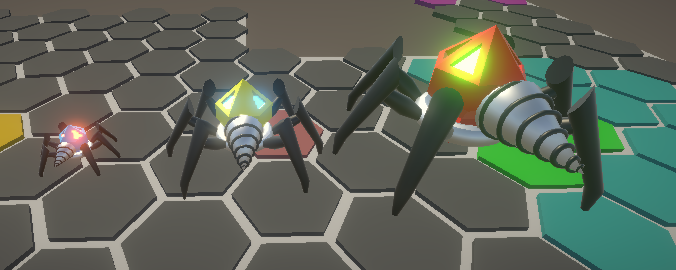
\includegraphics[width=1\textwidth]{Melee.png}
		\caption{Inamicul de lupta apropiată}
		\label{fig: enemyMelee}
	\end{figure}

	\begin{figure}[H]
		\centering
		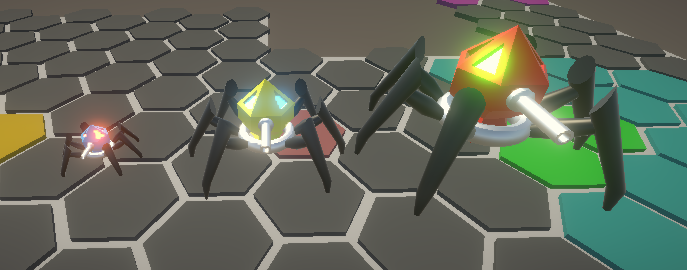
\includegraphics[width=1\textwidth]{Ranged.png}
		\caption{Inamicul de lupta de la distanță}
		\label{fig: enemyRanged}
	\end{figure}
	
	\begin{figure}[H]
		\centering
		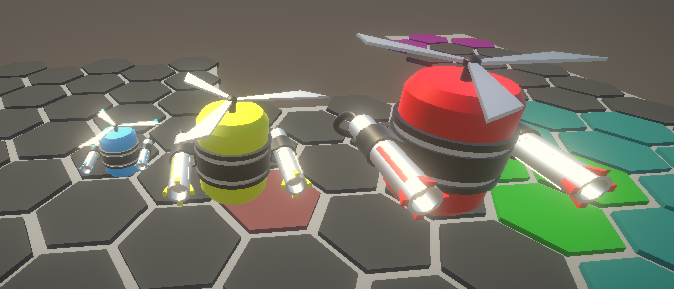
\includegraphics[width=1\textwidth]{Flying.png}
		\caption{Inamicul zburător}
		\label{fig: enemyFlying}
	\end{figure}
	
	\begin{figure}[H]
		\centering
		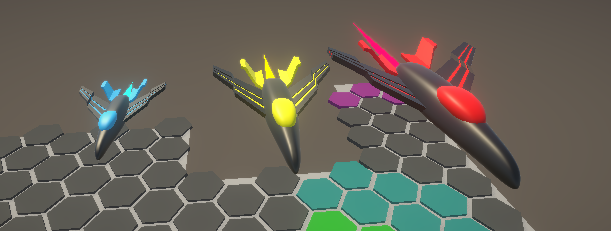
\includegraphics[width=1\textwidth]{Ambusher.png}
		\caption{Inamicul bombardier}
		\label{fig: enemyAmbusher}
	\end{figure}
	
	
	
	\subsubsection{Turnuri defensive}
	În continuare voi scrie o descriere scurtă pentru fiecare turn din joc. Toate proprietățile despre care urmează să vorbesc sunt în comparație cu celelalte turnuri defensive.
	\begin{itemize}
		\item \textbf{Serenity} (fig: \ref{fig: serenity}) este baza jucătorului. Are viață foarte multă, iar dacă este distrusă jucătorul pierde nivelul curent. Aceasta poate ataca inamicii care se apropie de ea. Are rază de atac medie, putere de atac mediu, poate ataca orice tip de inamic, iar rata de reîncărcare între atacuri este mică (durează mult timp între atacuri)
		\item \textbf{Mitralieră automată} (fig: \ref{fig: machineGun}) Are viața mică, poate ataca orice tip de inamic, are raza medie, putere de atac mică și rata de atac este mare (atacă foarte des)
		\item \textbf{Gardul electric} (fig: \ref{fig: electricFence}) este turnul de protecție. Are viață foarte mare, poate ataca doar inamicii de luptă apropiată, puterea de atac este medie, iar rata de reîncărcare este mică. Scopul acestui turn este să stea în calea inamicilor pentru a fi atacat de aceștia, permițând celorlalte turnuri să atace inamicii blocați.
		\item \textbf{Vulkan} (fig: \ref{fig: vulkan}) Este turnul special construit pentru a lupta împotriva inamicilor zburători. Are viață puțină, rază de atac mare și putere de atac mare dar poate ataca doar inamicii zburători.
		\item \textbf{Aruncătorul de flăcări} (fig: \ref{fig: machineCannon}). Când inamicii intră în rază acestui turn, el va împrăștia flăcări către inamici. Toți inamicii care intră în aceste flăcări primesc damage în fiecare clipă în care stau în flăcări. Are viață medie, atacă instant și puterea de atac este mică dar distribuită în fiecare clipă în care inamicii stau în flăcările acestuia.
		\item \textbf{Laser} (fig: \ref{fig: railgun}). Este un turn similar cu aruncătorul de flăcări în sensul în care atacă în fiecare clipă în care un inamic este în raza acestuia. Atacă cu un laser puternic care scade treptat viața inamicilor. Are viață medie, atacă instant și puterea de atac este mică.
		\item \textbf{Excavator} (fig: \ref{fig: excavator}) este un tip special de turn deoarece nu poate ataca inamicii. Acesta adună resurse în timpul luptei, resurse care pot fi convertite în bani de joc. Are viață multă, și pentru că nu poate ataca, trebuie să fie aparat de inamici.
	\end{itemize}
	
	\begin{figure}[H]
		\centering
		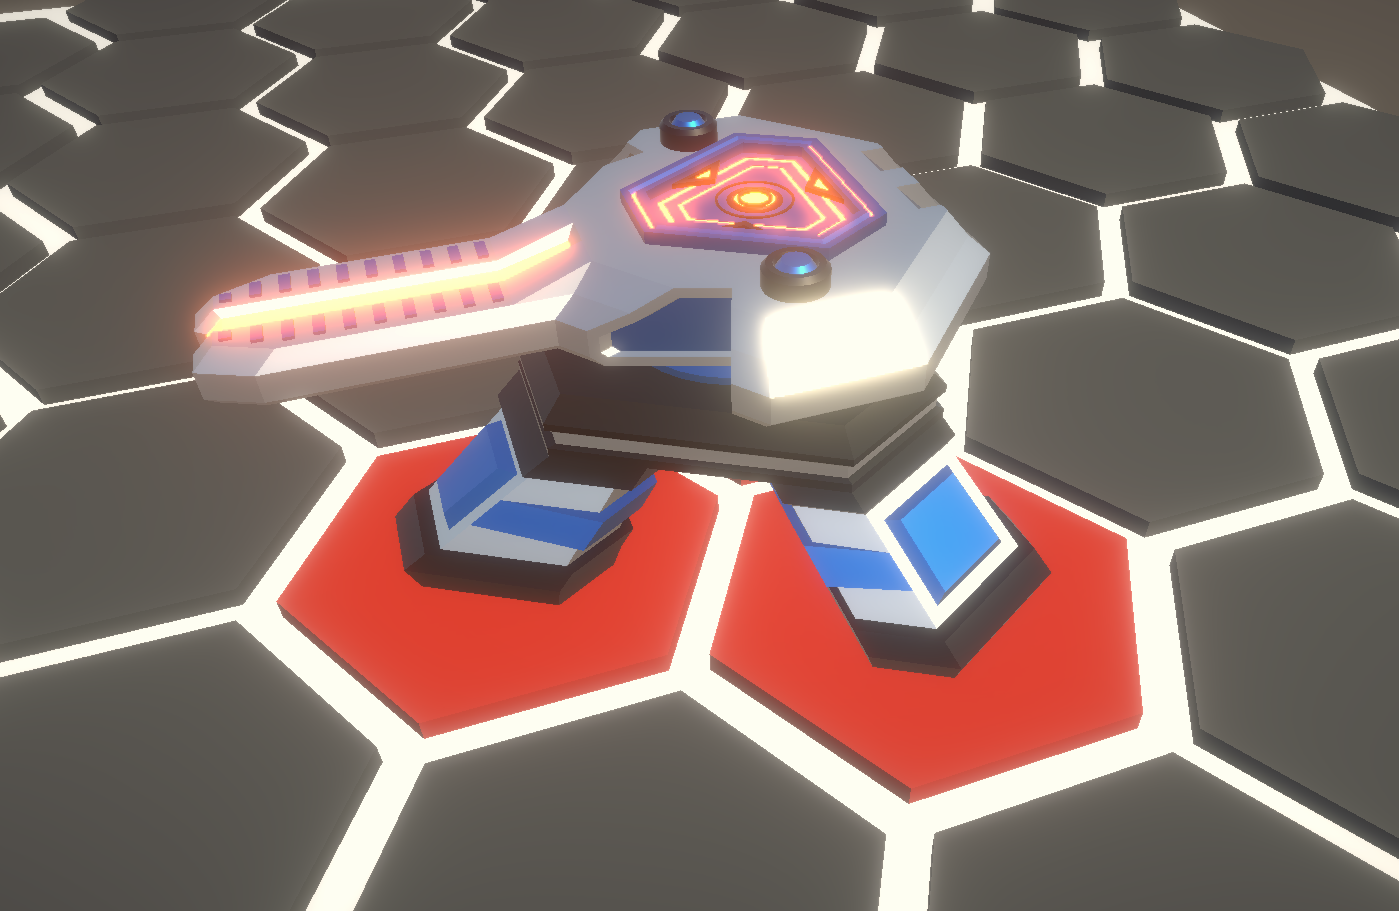
\includegraphics[width=1\textwidth]{Serenity.png}
		\caption{Serenity}
		\label{fig: serenity}
	\end{figure}
	
	
	\begin{figure}[H]
		\centering
		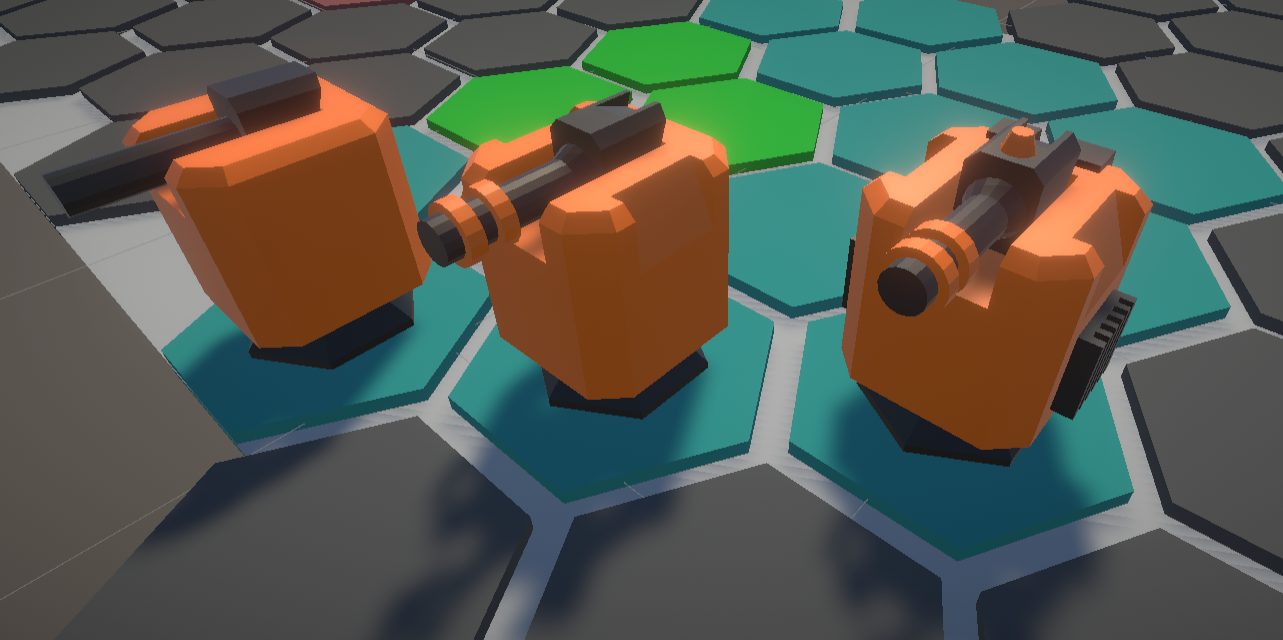
\includegraphics[width=1\textwidth]{machineGun.png}
		\caption{Mitraliera automata}
		\label{fig: machineGun}
	\end{figure}

	\begin{figure}[H]
		\centering
		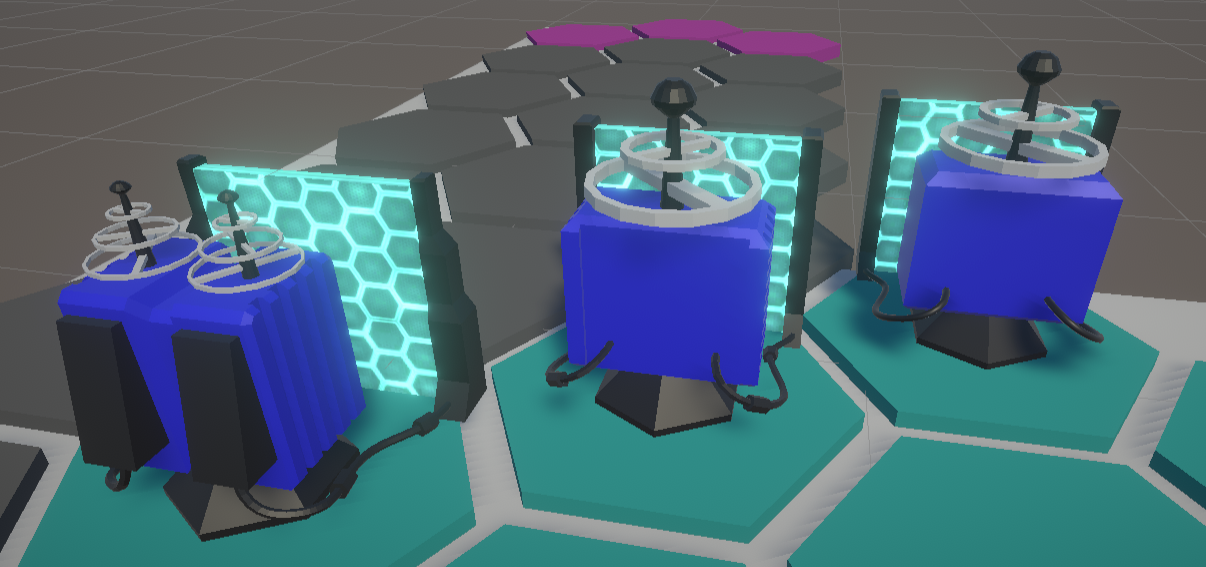
\includegraphics[width=1\textwidth]{electricFence.png}
		\caption{Gardul electric}
		\label{fig: electricFence}
	\end{figure}

	\begin{figure}[H]
		\centering
		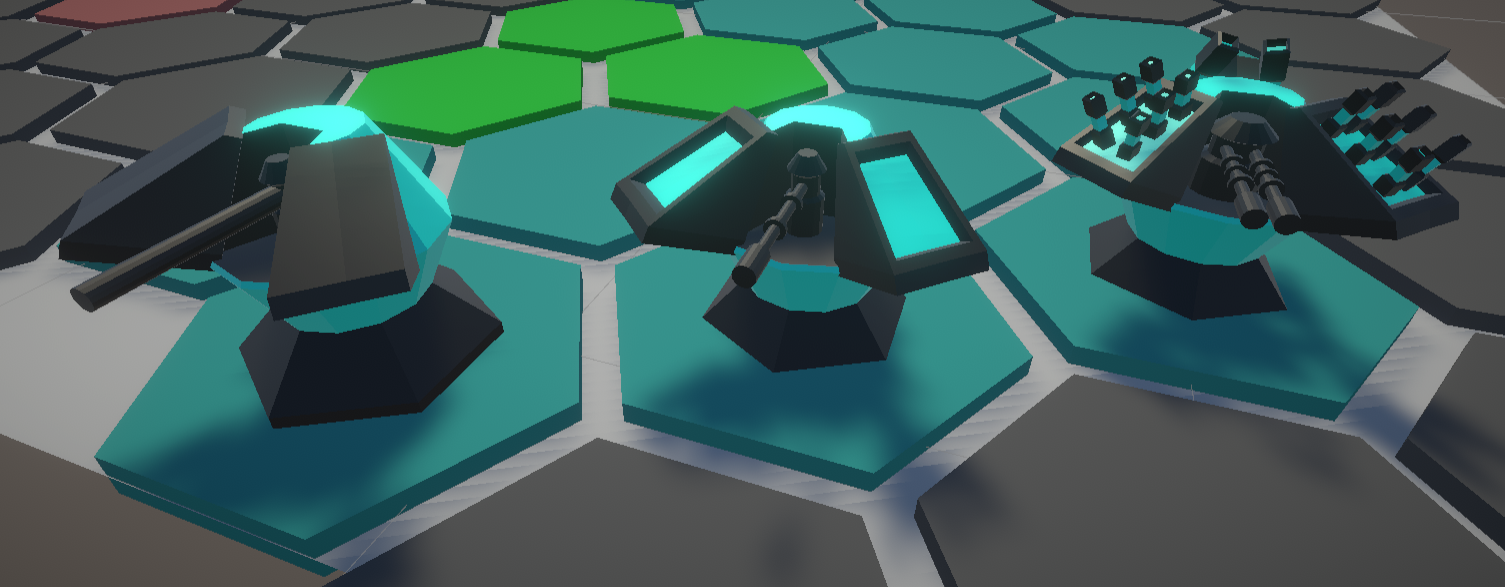
\includegraphics[width=1\textwidth]{vulkan.png}
		\caption{Vulkan}
		\label{fig: vulkan}
	\end{figure}

	\begin{figure}[H]
		\centering
		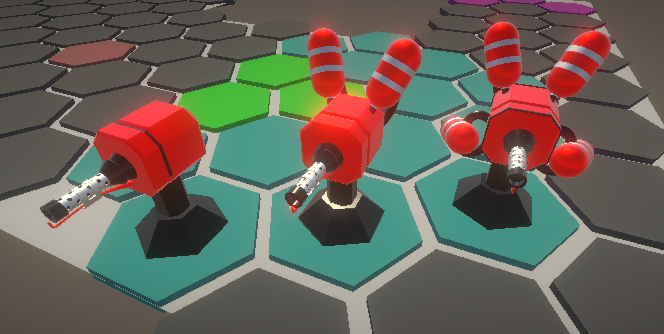
\includegraphics[width=1\textwidth]{Flamethrower.png}
		\caption{Aruncatorul de flacari}
		\label{fig: machineCannon}
	\end{figure}
	
	\begin{figure}[H]
		\centering
		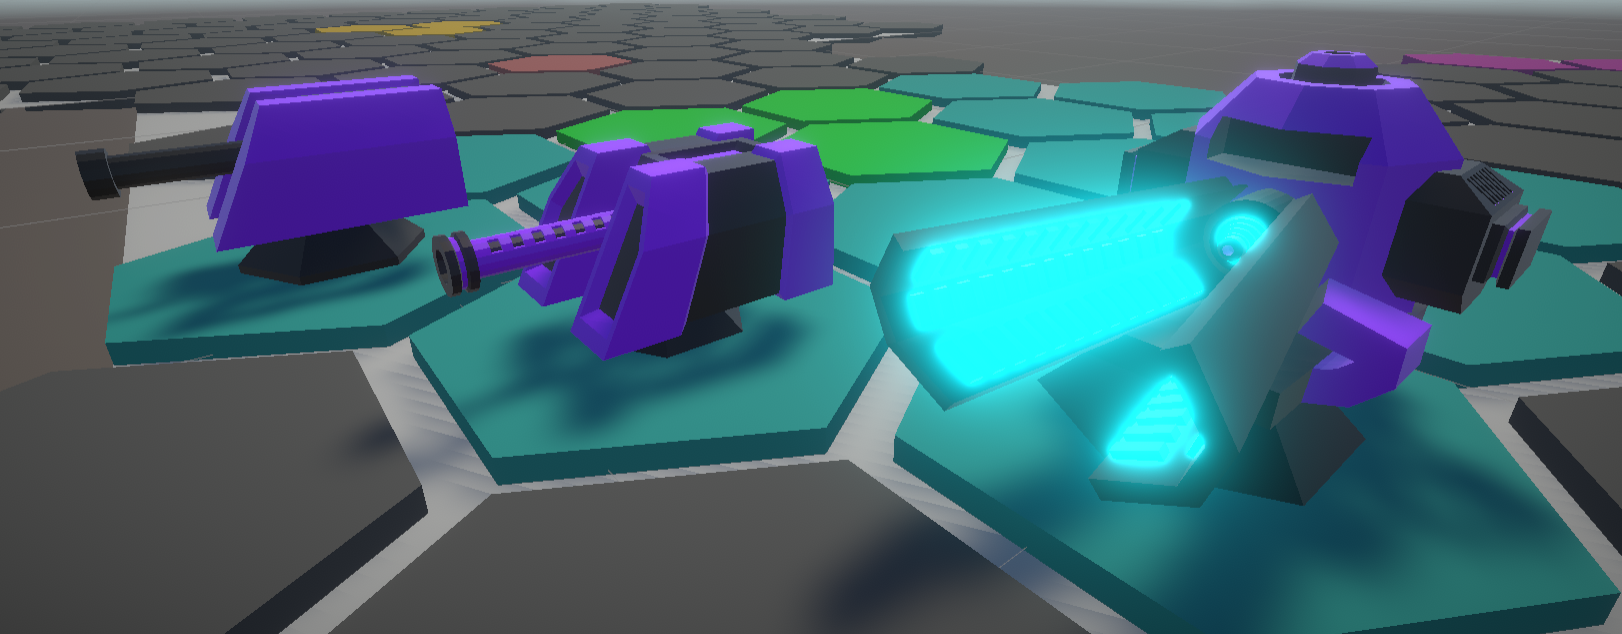
\includegraphics[width=1\textwidth]{railgun.png}
		\caption{Laser}
		\label{fig: railgun}
	\end{figure}

	\begin{figure}[H]
		\centering
		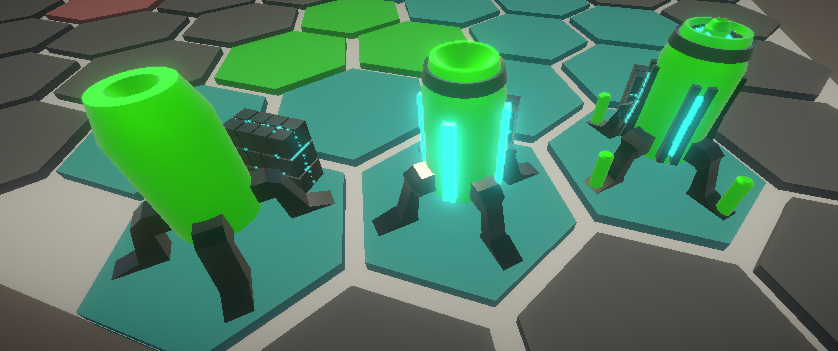
\includegraphics[width=1\textwidth]{Excavator.png}
		\caption{Excavator}
		\label{fig: excavator}
	\end{figure}
	
	
	
	
	
	\subsection{Sistemele Jocului}
	
	\subsubsection{Harta de joc}
	
	Pe hara jocului vor fi generate automat obiecte hexagonale. Aceste obiecte pot fi de mai multe tipuri:
	\begin{itemize}
		\item Hexagoane goale (cele gri din (fig: \ref{fig: gridSystem})).
		\item Hexagoane pe care putem construii turnuri de atac. (cele albastre din fig: \ref{fig: gridSystem})
		\item Hexagoane pe care putem construii turnul de extragere de resurse. (cele verzi din fig: \ref{fig: gridSystem})
		\item Hexagonul pe care va începe și se va afla comandantul. (cel roz din fig: \ref{fig: gridSystem})
		\item Hexagoanele bazei jucătorului. Baza va ocupa 3 hexagoane de acest tip. (cele galbene din fig: \ref{fig: gridSystem})
		\item Hexagonul ocupat. Fiecare hexagon care este ocupat de o anumită structura devine un astfel de hexagon. (are culoarea roșie)
	\end{itemize}
	
	Inamicii vor calcula drumul pe care merg în funcție de toate aceste tipuri de hexagoane. Din acest motiv este nevoie și de cel gol.
	
	\begin{figure}[H]
		\centering
		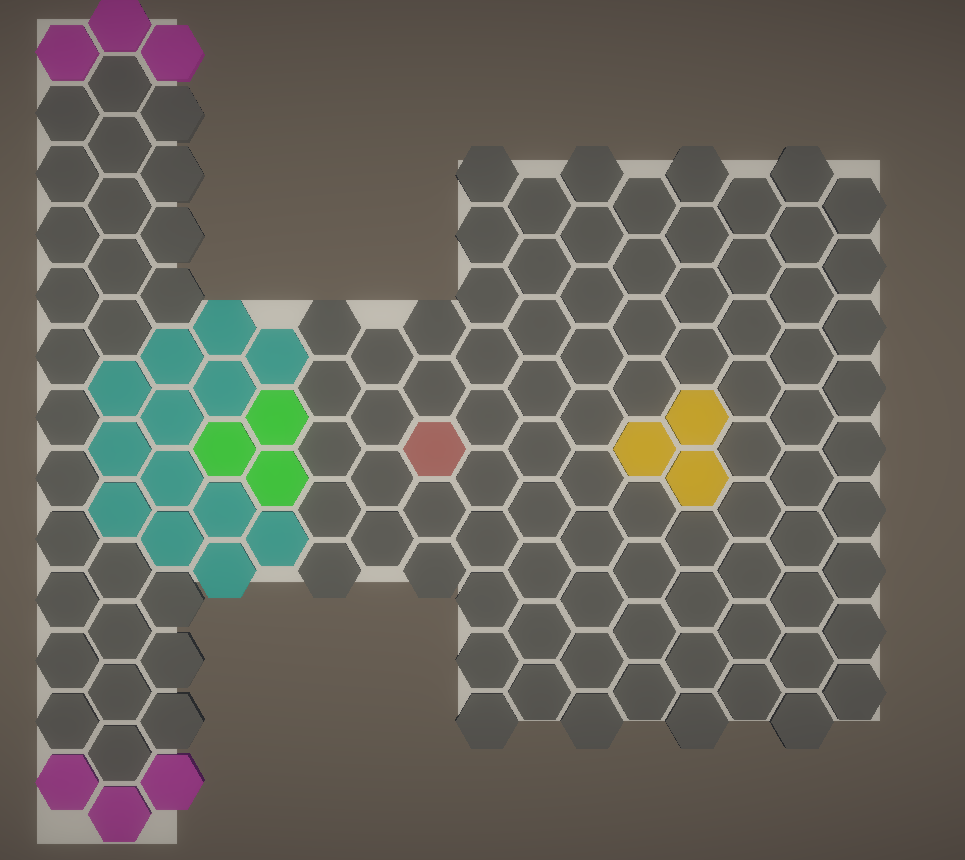
\includegraphics[width=1\textwidth]{Map.png}
		\caption{Harta de joc}
		\label{fig: gridSystem}
	\end{figure}


	
	
	
	\subsubsection{Sistemul Turnurilor}
	
	Turnurile pot fi plasate doar pe hexagoanele de construcție. Odată plasate, acestea nu pot fi mutate. Singurele metode de a goli acel hexagon sunt să fie distrus de un inamic sau să vindem turnul respectivă. Dacă vindem un turn, vom primii înapoi o parte din banii investiți, bani cu care putem să îmbunătățim celelalte turnuri. Toate turnurile au următoarele proprietăți:
	\begin{itemize}
		\item Viteză de atac
		\item Putere de atac
		\item Viață
		\item Rază de atac
		\item Inamicii pe care pot să îi atace
	\end{itemize}
	
	Dacă viață turnului ajunge la 0, va fi distrus automat. Atâta timp cât un turn nu este distrus, îl putem repara, dar reparațiile vor fi executate într-un anumit interval de timp, timp în care turnul nu va putea ataca dar va putea în continuare să fie atacat de inamici.
	
	
	
	
	
	\subsubsection{Comandantul}
	
	Comandantul poate fi mutat pe orice hexagon care nu este deja ocupat. După ce ai ales un hexagon, acesta va începe să se miște către acea locatie. Cât timp este în mișcare, nu poate să atace inamicii. Destinația poate fi schimbată doar după ce a ajuns la destinația selectată. Are rază medie, rată de atac medie, putere de atac mediu și poate ataca orice tip de inamic. Acesta poate întra în turnuri, îmbunătățindu-le exponențial proprietățile.
	
	
	
	\subsubsection{Valul de inamici}
	
	Jocul va avea mai multe nivele, care pot fi selectate dintr-un meniu, acestea fiind cât mai diversificate posibil. Inamicii au mai multe puncte din care pot să vină în funcție de nivelul ales. Aceștia vin în grupuri de inamici, între fiecare grup existând o perioada de repaus în care jucătorul își poate repara turnurile. În caz că nu are nevoie de reparații, poate selecta să sară peste perioada de repaus, astfel primind bani extra.
	
	
	
	
	
	\subsubsection{Nivelele jocului}
	
	Nivelul este terminat când toți inamicii au fost omorâți. Fiecare nivel va avea un scor de maxim 3 stele, care specifică cât de bine s-a descurcat la acest nivel. Scorul este calculat în funcție de viață rămasă a bazei la finalul nivelului. Fiecare stea câștigată va da bani extra, bani care pot fi folosiți în magazinul de îmbunătățiri permanente, despre care vom discuta în scurt timp.
	\newline
	
	Jucătorul poate să joace din nou nivelele, dar nu va mai primii atât de mulți bani ca prima dată. Acesta va câștiga bani extra de pe stelele obținute doar dacă a primit mai multe stele decât turele anterioare.
	
	
	
	
	
	\subsubsection{Lock-on}
	
	Jucătorul poate să apese pe inamici, astfel setand acel inamic drept o prioritate. Fiecare turn care poate ataca acest tip de inamic îl va prioritiza față de alți inamici. De îndată ce este omorât, se pierde această prioritate.
	
	
	
	
	
	\subsubsection{Magazinul de îmbunătățiri permanente}
	
	Între nivele putem să cumpărat piese de schimb pentru turnurile noastre pentru a le face mai puternice. Aceste piese se pot cumpăra doar cu banii câștigați de pe urmă nivelelor. Îmbunătățirile pt fiecare tureta în parte sunt următoarele:
	
	\begin{itemize}
		\item Mitralieră automată: atac mai puternic, rază de atac mai mare, rată de atac mai mare.
		\item Gardul electric: mai multă viață, atac mai puternic, rată de atac mai mare.
		\item Vulkan: atac mai puternic, rază de atac mai mare, atac mai rapid
		\item Aruncătorul de flăcări: atac mai puternic, rază de atac mai mare, viață mai multă.
		\item Laser: atac mai puternic, rază de atac mai mare, viață mai multă.
		\item Excavator: mai mulți bani, timpul între livrările de bani mai scurt, viață mai multă.
	\end{itemize}
	
	Fiecare îmbunătățire va avea mai multe nivele, fiecare costând din ce în ce mai mulți bani, dar vor avea un nivel maxim la care putem duce aceste îmbunătățiri.
	
	
	
	
	
	\subsubsection{Raid system}
	
	Când un jucător alege acest mod, este dus la o pagină de login în care trebuie să își specifice numele sau să îl păstreze pe cel generat automat. După ce intră în cont, trebuie să intre într-o cameră de așteptare. Ca să intre într-o cameră de așteptare, poate să creeze el una, să aleagă dintr-o listă cu toate camerele existente sau să între automat într-una existentă, care este aleasă aleator. În cazul ultimei opțiuni, dacă nu există nici o cameră libera, acesta se creează automat. 
	\newline
	
	În urma intrării în cameră, poate să selecteze dificultatea nivelului, iar de îndată ce toți jucătorii din cameră sunt gata, pot să inceapă nivelul.
	\newline
	
	În centrul hărții se află un monstru imens de foc. Scopul nivelului este să învingi monstrul împreună cu coechipierul tău, înainte ca monstrul să distrugă baza vreunuia dintre jucători.
	\newline
	
	Fiecare jucător poate plasa turnuri oriunde, putând să îmbunătățească, repare sau vinde doar turnurile construite de el. Amândoi jucătorii au caracterele lor comandant, dar aceștia nu pot întra în acelasi turn în același timp. Pentru sistemul de lock-on, doar turnurile jucătorului care a setat lock-on-ul va ataca inamicul prioritizat.
	
	
	
	
	
	\subsubsection{Atacurile monstrului de foc}
	
	Monstrul de foc are o serie de atacuri predefinite care devin mai puternice în dificultățile avansate.
	
	\begin{itemize}
		\item Abilitatea automată: crește puterea de atac pe măsură ce pierde din viață.
		\item Ploaia de meteoriți: ridică o mâna sus și generează meteoriți unul după altul. Fiecare meteorit când este construit complet alege un turn și pornește către direcția acestuia. Când se izbește de turn explodează și scade din viață turnului în funcție de dificultatea selectată.
		\item Gheară invartitoare: se învârte 360 grade și lovește toate turnurile de pe hartă cu mâna lui dreapta.
		\item Meteoritul suprem: când ajunge la un anumit procentaj de viață începe acest atac. Alege una dintre bazele jucătorilor (în caz că sunt mai mulți), se rotește spre baza selectată și începe să încarce un meteorit imens. Încărcarea acestuia durează 30 de secunde, iar dacă în acest timp jucătorul reușește să îi scadă suficient de mult viața monstrului, atacul este întrerupt și devine confuz timp de 10 secunde, timp în care poate fi atacat neîntrerupt. Dacă jucătorii nu reușesc să îi scadă suficient de mult viață, va lovii puternic cu meteoritul baza selectată și turnurile din jur.
	\end{itemize}
	
	Toate interacțiunile acestui nivel sunt sincronizate în rețea prin utilizarea modulului Photon Engine.
	
	
	
	
	
	\subsection{Analiza proiectului din punctul de vedere al consumatorilor}
	
	\subsubsection{Dificultatea jocului}
	
	Jocul va fi relativ dificil. Jucătorul trebuie să se gandesca unde să construiesca anumite turnuri pentru a folosi resursele cât mai bine. La început jocul va fi ușor, dar pe măsură ce progresează, nivelele vor devenii din ce în ce mai dificile. Trebuie să se gandesca și dacă poate rezista să sară peste perioada de repaus între grupurile de inamici.
	\newline
	
	Sistemul co-op are un nivel de dificultate cu mult mai ridicat, pentru că trebuie să se gândească cum să se coordoneze cât mai bine cu coechipierul.
	
	
	
	
	
	\subsubsection{Elemente de dependență}
	
	În caz că nu putem depasii un anumit nivel, putem juca nivelele anterioare și să ne asigurăm că obținem 3 stele la fiecare nivel. Această metodă de a obține 3 stele la fiecare nivel poate fi unul din motivele care îi determina pe jucători să continue să joace jocul. Un alt factor ar putea fi sistemul de îmbunătățiri permanente.
	
	
	
	
	
	\subsubsection{Grupele de vârstă vizate}
	
	Acest joc nu are limitări de vârstă, poate fi jucat de oricine, dar va fi apreciat cel mai mult de copii și de adolescenții care caută provocări în jocurile de strategie. Jocul este în principiu făcut pentru jucătorii ocazionali de jocuri video.
	
	
	
	
	
	\section{Implementarea proiectului}
	\label{section: projectImplementation}
	
	\subsection{Scena de luptă}
	
	\subsubsection{Inițializarea scripturilor}
	\label{section: initialization}
	
	În Unity scripturile au câteva metode care ajută la inițializare.
	\newline
	
	\textbf{Awake} este metoda care este apelată la începutul programului și înainte de restul metodelor.
	\newline
	
	\textbf{Start} este metoda care este apelată după ce au fost apelate metodele "Awake" de la toate scripturile.
	\newline
	
	\textbf{Update} este apelat la fiecare cadru al jocului, aici intervenind o mare parte din logică jocurilor. Apelarea update-ului începe după ce toate metodele "Start" au fost apelate.
	\newline
	
	Pentru "Start" și "Awake", unity decide automat în ce ordine să le apeleze, fără că noi să putem controla acest lucru. În multe proiecte mai complexe se ajunge în momentul în care, pentru initializatea anumitor sisteme este necesar ca alte sisteme să fie deja inițializate. Cum nu putem controla ordinea de inițializare, se ajunge în punctul în care putem primi erori aleatorii din cauza inițializării haotice.
	\newline
	
	Pentru a combate acest lucru, m-am gândit la un sistem care va permite controlarea inițializării tuturor acestor procese cu ușurință.
	
	\begin{figure}[H]
		\centering
		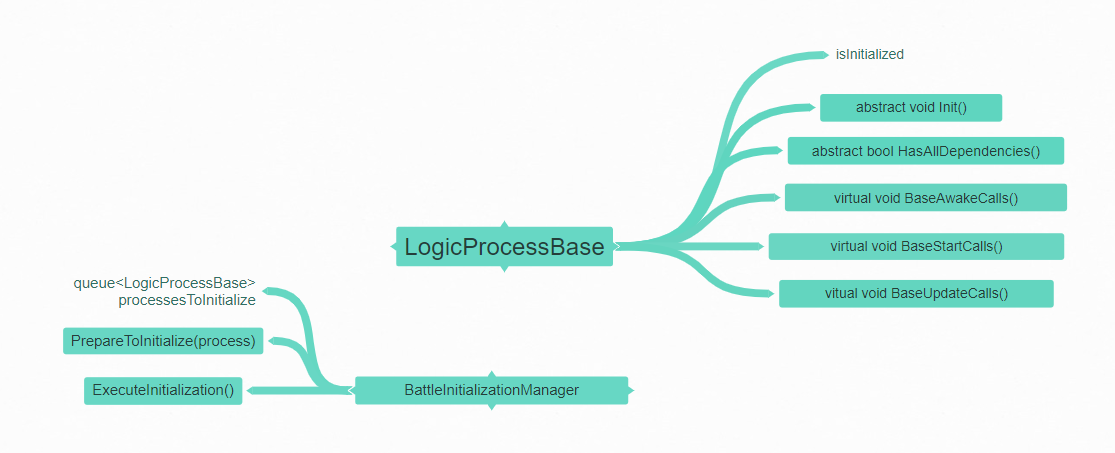
\includegraphics[width=1\textwidth]{logicProcessCoggle.png}
		\caption{Inițializarea scripturilor}
		\label{fig: logicProcessCoggle}
	\end{figure}
	
	Am creat clasa LogicProcessBase care ajută în acest proces. Fiecare script care necesită o inițializare mai organizată trebuie să o moștenească. Aceasta conține:
	\begin{itemize}
		\item \textbf{isInitialized} care specifică dacă scriptul curent a fost initializat sau nu încă
		\item \textbf{Init()}. În această metodă trebuie să scriem tot codul de inițializare a clasei care moștenește.
		\item \textbf{HasAllDependencied()}. Este o metodă care returnează un boolean. În această clasa trebuie să punem toate dependințele de care are nevoie clasa care moștenește.
		\item \textbf{BaseAwakeCalls()}. În această metodă apelăm "PrepareToInitialize()" din clasa "BattleInitializationManager", despre care vom vorbi în scurt timp.
		\item \textbf{BaseStartCalls()} și \textbf{BaseUpdateCalls()} sunt metode în care trebuie să scriem tot codul care normal ar fi venit în Start/Update. În unity, nu putem defini Start/Update drept virtual și să modificăm funcțiile lor pe urmă, din acest motiv tot codul din clasele dintr-o ierarhie mai complexă trebuie să fie scris în aceste metode, iar în clasa cel mai jos din ierarhie trebuie să le apelăm în Awake/Start/Update.
	\end{itemize}
	
	\textbf{BattleInitializationManager} este a două clasa de care avem nevoie. Ea este responsabilă pentru a executa initializarea propriu-zisă a proceselor. 
	\newline
	
	\textbf{PrepareToInitialize()} este apelată de fiecare proces în metoda lor de Awake, iar această metodă va adăuga procesul într-o coadă.
	\newline
	
	\textbf{ExecuteInitialization()} parcurge toate procesele din coadă și verifică dacă acestea pot fi initializate, apelând "HasAllDependencies()". Dacă procesul curent poate fi initializat, atunci apelează metoda Init() și setează "isInitialized = true". Dacă nu îl poate inițializă, îl adaugă la finalul cozii pentru a fi initializat la final. Acest proces se repetă până când coadă este goală sau s-a parcurs o dată coada cap-coadă și nu s-a initializat nici un proces. În acest caz înseamnă că aveau dependințe circulare și oprim procesul de inițializare, afișând un mesaj de eroare. Această metodă trebuie apelata în Awake, Start și Update, deoarece, pe parcurs pot apărea noi procese care trebuie initializate, iar programul trebuie să poată să detecteze astfel de cazuri.
	
	
	
	
	
	\subsubsection{Procesarea comenzilor venite de la utilizator}
	
	O altă problema des întâmpinată în proiectele mari este procesarea comenzilor venite de la utilizator. În cazul în care procesăm comenzile în mai multe script-uri, când dorim să schimbăm modul în care funcționează comenzile sau să schimbăm platforma pe care rulează jocul, va trebuii să schimbăm toate scripturile în care procesăm comenzile utilizatorului. În proiectele mari, acest lucru duce la mult timp pierdut și din acest motiv m-am gândit la o metodă de a organiza mai bine acest sistem.
	\newline
	
	Ideea propusă de mine este să păstrăm toată procesarea de comenzi ale utilizatorului într-un singur script. Acest script are definite evenimente/delegate pentru toate tipurile de input specifice. Alte scripturi se pot abona la aceste evenimente, iar când utilizatorul apasă tasta respectivă, toate metodele abonate la evenimentul respectiv vor fi apelate.
	\newline
	
	Pe lângă asta, este necesar să știm și anumite informații legate de comanda primită la utilizator. Informațiile adiționale de care am avut nevoie sunt:
	
	\begin{itemize}
		\item Poziția pe ecran la care a fost apăsat mouse-ul/ecranul (în cazul rulării pe android)
		\item Poziția pe ecran la care a fost ridicată apăsarea mouse-ului/ecranului (în cazul rulării pe android)
		\item Dacă în clipă curentă este sau nu apăsat mouse-ul/ecranul
		\item Timpul la care a fost apăsat mouse-ul/ecranul
		\item Timpul la care a fost ridicată apăsarea mouse-ului/ecranului
		\item Obiectul pe care utilizatorul a dat click în scenă. În momentul când apăsăm click, se creează un Raycast care are ca origine poziția mouse-ului pe ecran și care se îndreaptă către scenă în perspectiva în care se află camera la clipă curentă. Acest Raycast detectează dacă a fost lovit un obiect, și dacă da, reținem care obiect a fost lovit pt ca alte scripturi să se poată folosi de această informație.
		\item Elementul cel mai de sus din ierarhia obiectului lovit. Datorită faptului că anumite modele au o structura complexă, uneori nu ne este deloc util să știm în mod direct ce obiect a fost lovit. De exemplu în caz că apăsăm peste un turn și Raycast-ul lovește pușcă turnului, nu ne va ajută deloc în cazul în care ne interesează să aflăm ce tip de turn am lovit. Din acest motiv, în clipa în care găsim obiectul pe care am dat click, reținem și părintele cel mai de sus din ierarhie.
	\end{itemize}
	
	Această organizare a procesării comenzilor ne permite să schimab tastele folosite cu ușurință și să adăugăm suport pentru dispozitive noi foarte ușor. În cazul dispozitivelor noi, putem folosi directive de unity pentru a separa codul specific pentru calculator de cel specific pentru android sau orice alt dispozitiv. Procesarea comenzilor în cele 2 cazuri vor fi diferite, dar datorită faptului că se invocă evenimentele deja definite, alte script-uri nu trebuie modificate absolut deloc.
	
	
	
	
	
	\subsubsection{Harta de joc}
	
	Acțiunea jocului se petrece pe o hartă care este formată din mai multe blocuri hexagonale. Această hartă este generată automat în funcție de ce tip de hartă alegem pentru nivelul respectiv. Înainte să începem să investigăm indetaliat sistemul hărții de joc, trebuie mai întâi să definim ce reprezintă un bloc hexagonal pe hartă.
	\newline
	
	
	
	
	
	\textbf{Blocul hexagonal}
	
	Pentru a reține informații specifice pentru un bloc, am definit clasa HexagonalBlock. În interiorul clasei am folosit de două enum-uri: \textbf{SpawnPointsID} și \textbf{HexagonType}.
	\newline
	
	HexagonType definește tipul blocului hexagonal și interacțiunile posibile cu acesta. Tipurile definite în acest enum sunt:
	
	\begin{itemize}
		\item \textbf{Walkable}. Blocul primește culoarea gri și toate creaturile pot să se deplaseze pe acesta.
		\item \textbf{TurretBuildable}. Blocul primește culoarea albastră și reprezintă zonele de pe harta unde putem să construim turnurile noastre.
		\item \textbf{ResourceExtraction}. Blocul primește culoarea verte și reprezintă zonele de pe harta în care putem construii turnul excavator.
		\item \textbf{Occupied}. Blocul primește culoarea roșie și reprezintă zonele în care este construit un turn sau locul în care se află comandantul.
		\item \textbf{SpawnPoint}. Blocul primește culoarea mov și reprezintă locul din care pornesc inamicii.
		\item \textbf{Impassable}. Blocul primește culoarea roșu închis și reprezintă locurile prin care nu pot să treacă inamicii. Sistemul de navigare va ignora toate aceste blocuri și va găsi rute alternative.
		\item \textbf{PlayerBase}. Blocul primește culoarea galbenă și reprezintă locul în care va fi creată baza jucătorului. Pentru ca un nivel să fie considerat valid, trebuie să existe 3 astfel de blocuri unul lângă altul.
		\item \textbf{CommanderSpawn}. Blocul primește culoarea mov și reprezintă locul în care va începe comandantul. Pentru ca un nivel să fie considerat valid, trebuie să existe exact o instanța a acestui bloc pe harta.
	\end{itemize}
	
	SpawnPointsID definește o serie id-uri pentru blocurile de tip SpawnPoint. În fișierul de configurare al valului de inamici, discutat în capitolul \ref{section: enemyWave}, putem specifica id-ul blocului de la care vor începe inamicii. În caz că, pentru un val de inamici specificăm ca inamicii să începă de la o locație aleatoare, atunci se va alege un bloc aleatoriu dintre toate blocurile de pe hartă.
	\newline
	
	Blocul hexagonal definește și o listă de materiale, care sunt folosite pentru a schimba culoarea blocului în momentul în care tipul acestuia se schimbă.
	\newline
	
	Are definite și 2 metode ajutătoare și anume PlaceHexagon(), care așează blocul pe harta în funcție de poziția și diametrul specificat în parametrii, și UpdateMaterial() care actualizează culoarea blocului, prin schimbarea materialului pe care îl folosește.
	\newline
	
	Pentru a pune în funcțiune schimbarea de culoare a blocului hexagonal direct din editor, a trebuit să creez clasa specială HexagonalBlockEditor. Această clasă moștenește clasa Editor, pentru a putea schimba interfața grafică a editorului din Unity. Această clasa, în metoda OnInspectorGUI care este apelată de fiecare dată când obiectul este selectat, verifică dacă s-a schimbat tipul blocului, și dacă da, atunci apelează metoda UpdateMaterial() de pe blocul selectat.
	\newline
	
	
	
	
	
	\textbf{Harta propriu-zisă}
	
	Clasa special definită pentru harta de joc este HexagonalGrid. Această clasa are câteva proprietăți publice care definesc dimensiunea hărții: diameter (care definește cât de mare este fiecare hexagon), offset (care este aplicat în așa fel încât hexagoanele vor fi poziționate la distanțe egale între ele) și mapScaleOffset (harta de joc este scalată automat la dimensiunea ecranului; acest offset ne ajută să scalăm harta mai mult sau mai puțin decât ar fi fost scalată automat).
	\newline
	
	Scriptul are definit o listă de tipul HexagonalBlock, care reține toate blocurile hexagonale de pe hartă și mai are definit o variabilă publică care reprezintă tipul de hartă pe care o folosim. Tipul de harta este reprezentat de un model 3D care va fi folosit pentru a poziționa hexagoanele.
	\newline
	
	Clasa moștenește LogicProcessBase, iar în metoda Init(), găsește fișierul de configurare al nivelului curent, discutat în capitolul \ref{section: stageScriptable}, șterge toate blocurile existente de pe hartă și citește fișierul de configurare al hărții (definit în fișierul de configurare al nivelului și explicat în secțiunea următoare). După ce a citit conținutul fișierului, apelează metoda SpawnAndScaleMap() și metoda LoadPresetGrid().
	\newline
	
	SpawnAndScaleMap() creează o instanță a hărții de joc (modelul 3d care este definit drept variabilă publică), găsește limitele acesteia în coordonate 3D, și în funcție de dimensiunea ecranului, scalează harta în așa fel încât să încapă harta în întregime pe ecran. Pe urmă, în funcție de mapScaleOffset, scaleaza din nou harta în funcție de dorința persoanei care a definit nivelul.
	\newline
	
	Înainte să vorbim despre funcția LoadPresetGrid() trebuie să discutăm despre CreateGrid(). Aceasta funcție se folosește de modelul 3D al hărții pentru a genera și poziționa toate blocurile hexagonale necesare. Această parcurge întreagă dimensiune a modelului 3D, și folosindu-se de fizică definită de Unity (Physics.Raycast), verifică dacă în poziția curentă de pe model a reușit să lovească suprafața. În caz că a reușit să lovească, atunci generează un bloc hexagonal, îl adaugă în listă și caută în continuare până când a reușit să parcurgă întreg modelul 3D. La final o să avem generate pe hartă blocuri hexagonale care sunt poziționate în toate zonele de pe modelul 3D al hărții, fiecare bloc fiind de tipul Walkable.
	\newline
	
	LoadPresetGrid() preia conținutul fișierului configurabil, apelează metoda CreateGrid(), după care începe să itereze peste fiecare element din blocurile generate. La fiecare iterație, inițializează blocul curent în funcție de datele din fișierul configurabil al hărții de joc, și în caz că întâlnește blocuri de tipul PlayerBase sau CommanderSpawn, generează și poziționează pe harta comandantul și baza jucătorului. În caz că fișierul este corupt, nu a găsit blocurile pentru comandant și penrtu baza jucătorului sau a găsit prea multe din acestea, afișează mesaje de eroare pentru fiecare caz în parte.
	\newline
	
	
	
	
	
	\textbf{Fișierul de configurare pentru harta de joc}
	
	Pentru a putea crea cu ușurință nivele cât mai variate, trebuie să reținem anumite date în fișiere configurabile. Aceste fișiere configurabile trebuie să fie făcute în așa fel încât prin încărcarea unui simplu fișier, putem genera un nivel de joc complet funcțional.
	\newline
	
	În acest scop am definit clasa GridSaveData, care reține proprietățile cele mai importante ale hărții de joc. Această clasa reține diametrul blocurilor, offset-ul și mapScaleOffset, pentru a putea încarcă harta la aceeași scala la care era configurată inițial. Pe lângă asta, reține o lista cu tipurile blocurilor hexagonale de pe hartă și id-urile setate pentru blocurile de pe care încep inamicii.
	\newline
	
	Această clasa este definită urmând o structura JSON, pentru a ușura serializarea și deserializarea datelor în momentul scrierii și citirii pe disk.
	\newline
	
	Pe lângă această clasa, am avut nevoie și de o clasa ajutătoare care să se ocupe de salvarea și încărcarea propriu-zisă a datelor. Clasa se numește GridDataSaver și este definită cu 2 metode statice simple: SaveData() și LoadData().
	\newline
	
	
	
	
	
	\textbf{Editorul special pentru crearea rapidă a nivelelor}
	
	Pentru a ușura generarea de nivele, am creat un editor cu funcții speciale. Clasa se numește HexagonalGridEditor și mostenteste clasa Editor din Unity. Folosind această clasa, am suprascris editorul implicit pentru clasa HexagonalGrid, iar în loc i-am adăugat câteva proprietăți ajutătoare. Am definit câmpuri publice pentru modelul 3D al hărții pentru care dorim să creăm un nivel, diametru, offset, mapScaleOffset și locația fișierului de configurare în care să salveze configurarea hărții și din care poate să încarce harta pentru a o modifică.
	\newline
	
	Pe lângă aceste câmpuri, am definit și câteva butoane care au că rol să apeleze funcționalități din scriptul HexagonalGrid. Fără aceste butoane, nivele ar fi putut fi create numai în timpul rulării aplicației, fapt ce nu era de dorit, deoarece este cu mult mai ușor să creăm hărți de joc direct din editor. Butoanele definite sunt: Scale Map, Reset Scale, Generate Grid, Clear Grid, Load Preset, Save Preset. Fiecare buton apelează funcționalitatea cu același nume din HexagonalGrid, exceptant Load Preset și Save Preset, care încarcă și salvează configurarea actuală a hărții în locația specificată prin câmpul public, folosindu-se de GridDataSaver.
	\newline
	
	Datorită acestui editor special, procesul de creare a hărților jocului a devenit foarte rapid. Pentru a crea o hartă nouă, trebuie să încărcăm un model 3D simplist definit într-un program de modelare 3D și să tragem acel model 3D în câmpul public de pe editor. Modificăm câmpurile de scalare a hărții și apăsăm pe butonul de Generate Grid repetat până când suntem mulțumiți de configurarea actuală. După acest lucru, selectăm blocurile hexagonale la care dorim să le schimbăm tipul. Datorită editorului HexagonalBlockEditor, culoarea acestora se schimbă automat, fapt care ne ușurează muncă enorm. După ce am definit toate tipurile blocurilor, specificăm locația la care dorim să salvăm fișierul de configurare al hărții și apăsăm pe butonul Save Preset.
	\newline
	
	În caz că dorim să modificăm configurarea unei hărți, specificăm locația fișierului de configurare a hărții respective. Setam câmpul modelului 3D cu modelul 3D pe care a fost generată inițial harta și apăsăm pe butonul Load Preset. După ce harta s-a încărcat cu succes, putem modifică blocurile hexagonale în modul dorit, iar când am terminat, apăsăm din nou pe butonul Save Preset pentru a suprascrie configurarea hărții.
	\newline
	
	
	
	
	
	\subsubsection{Sistemul de navigare}

	\begin{figure}[H]
		\centering
		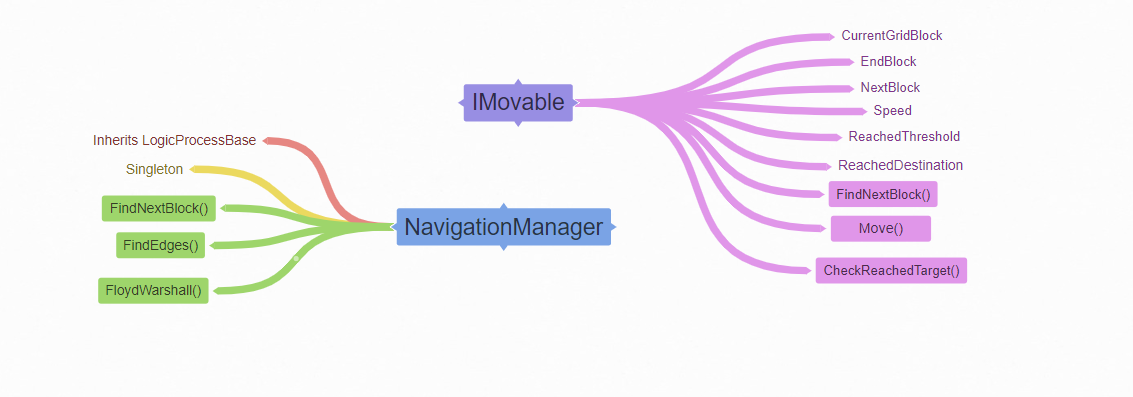
\includegraphics[width=1\textwidth]{navigationCoggle.png}
		\caption{Sistemul de navigare}
		\label{fig: navigationManager}
	\end{figure}

	Caracterele jocului trebuie să știe pe unde pot să se deplaseze ca să ajungă la o anumită destinație. În acest scop a trebuit să aleg un algoritm care să găsească cel mai scurt drum posibil. Am avut de ales între mai mulți algoritmi specifici, precum: Dijkstra, A*, Floyd-Warshall, etc.
	\newline
	
 	În cele din urmă am ales să folosesc Floyd-Wharshall. Acest algoritm are complexitatea $O(n^3)$ și presupune construirea celor mai scurte drumuri posibile pornind de la oricare nod către oricare alt nod din rețea. Deoarece construirea drumului se realizează doar la începutul jocului și reconstruirea acestui drum se realizează aproape instantaneu, am ales să folosesc acest algoritm.
	\newline
	
	"Considerăm rețeaua orientată $G = (N, A, b)$ reprezentată prin matricea valoare adiacentă $B = (b_{ij}), i, j \in N$ cu
	
	\begin{equation*}
		b_{ij} = \begin{cases}
			b(i, j) \quad daca \quad i \neq j \quad si \quad (i, j) \in A; \\
			0 \quad daca \quad i = j; \\
			\infty \quad daca \quad i \neq j \quad si \quad (i, j) \neq A.
		\end{cases}
	\end{equation*}

	Algoritmul Floyd-Warshall determina matricea distanțelor $D = (d_{ij}), i, j \in N$ și matricea predecesor $P = (p_{ij}), i, j \in N$." \cite{grafuriAnul2}
	
	\begin{algorithmic}
		\Function{Floyd-Warshall}{}
			\For{i $\gets$ 1 to n}
				\For{j $\gets$ 1 to n}
					\State $d_{ij} \gets b_{ij};$
					\If{i $\neq$ j and $d_{ij} < \infty$}
						\State $p_{ij} = i;$
					\Else
						\State $p_{ij} = 0;$
					\EndIf
				\EndFor
			\EndFor
			
			\For{k $\gets$ 1 to n}
				\For{i $\gets$ 1 to n}
					\For{j $\gets$ 1 to n}
						\If{$d_{ik} + d_{kj} < d_{ij}$}
							\State $d_{ij} = d_{ik} + d_{kj};$
							\State $p_{ij} = p_{kj};$
						\EndIf
					\EndFor
				\EndFor
			\EndFor
		\EndFunction
	\end{algorithmic}

	\begin{algorithmic}
		\Function{Reconstruire Drum}{}
			\State k = n;
			\State $x_k = j$
			\While{$x_k \neq i$}
				\State $x_{k - 1} = p_{ix_k};$
				\State k = k - 1
			\EndWhile
		\EndFunction
	\end{algorithmic}

	Drumul minim este $D_{ijp} = (x_k, x_{k+1}, \dots, x_{n-1}, x_n) = (i, x_{k+1}, \dots, x_{n-1}, j)$
	
	
	
	
	
	\subsubsection{Interfețe folosite}
	
	Pentru că o serie de obiecte din joc trebuie să urmeze aceleași concepte, am decis să mă folosesc de interfețe pentru a le definii modul în care trebuie să funcționeze. 
	\newline
	
	\textbf{IMovable}
	
	Deoarece inamicii și comandantul se pot mișca pe hartă, am creat această interfață pentru a defini aceleași concepte pentru toate caracterele care au nevoie să se miște pe hartă. Interfața se folosește de sistemul de navigare definit anterior și conține următoarele:
	
	\begin{itemize}
		\item Nodul curent la care se află.
		\item Nodul destinație.
		\item Nodul următor la care trebuie să se mute ca să se apropie de destinație.
		\item Vitezăa de deplasare.
		\item Distanță față de următorul nod pentru care considerăm că am ajuns la acesta. Deoarece lucrăm cu obiecte în spațiu 3D, este nevoide de o asemenea valoare.
		\item Un boolean care definește dacă am ajuns sau nu la destinație.
		\item O metodă care setează nodul următor la care trebuie să ajungem ca să ne apropiem de destinație. Acesta face apel la matricea construită de sistemul de navigare.
		\item O metodă care mișcă propriu-zis obiectul către următorul nod.
		\item O funcție care verifică dacă am ajuns sau nu la destinație.
	\end{itemize}
	\bigskip
	
	
	\textbf{IAttacker}
	
	Este o interfață pe care toate obiectele/caracterele care doresc să atace alte obiecte trebuie să o mostendeasca. Această conține următoarele date:
	
	\begin{itemize}
		\item Obiectul pe care trebuie să îl atace. Tipul este definit la moștenirea clasei datorită șablonului definit pentru interfață.
		\item Puterea de atac.
		\item Raza de atac.
		\item Durata între atacuri.
		\item Timpul la care s-a executat ultimul atac.
		\item Intervalul de timp între care se caută un nou inamic.
		\item Metoda care afișază/ascunde raza obiectelor din scenă. Raza acestora a fost defnita într-un shader special creat în Shader Graph.
		\item O metodă care caută cel mai apropiat inamic dacă există în rază.
		\item Metoda de atac pe care fiecare obiect o implementează diferit.
	\end{itemize}
	\bigskip
	
	\textbf{IDestroyable}
	
	Fiecare obiect care are o viață anume și care poate fi distrus trebuie să moștenească această interfață. Această conține următoarele date:
	
	\begin{itemize}
		\item Viața obiectului.
		\item Banii primiți când obiectul este distrus
		\item O metodă care distruge obiectul respectiv când viața lui a ajuns la 0.
	\end{itemize}
	\bigskip
	
	\textbf{IRecoverable}
	
	Turnurile pot să își refacă viața, iar ca un concept pentru viitor, ar putea să existe și anumiți inamici care refac viața altor inamici. Interfața conține următoarele date:
	
	\begin{itemize}
		\item Câtă viață se reface în fiecare secundă când efectul este aplicat.
		\item Costul refacerii în cazul în care este de dorit un cost.
		\item Un boolean care verifică dacă se reface sau nu în clipă curentă.
		\item O metodă care pornește procesul de refacere.
	\end{itemize}
	
	
	
	
	
	\subsubsection{Ierarhia inamicilor}
	
	\begin{figure}[H]
		\centering
		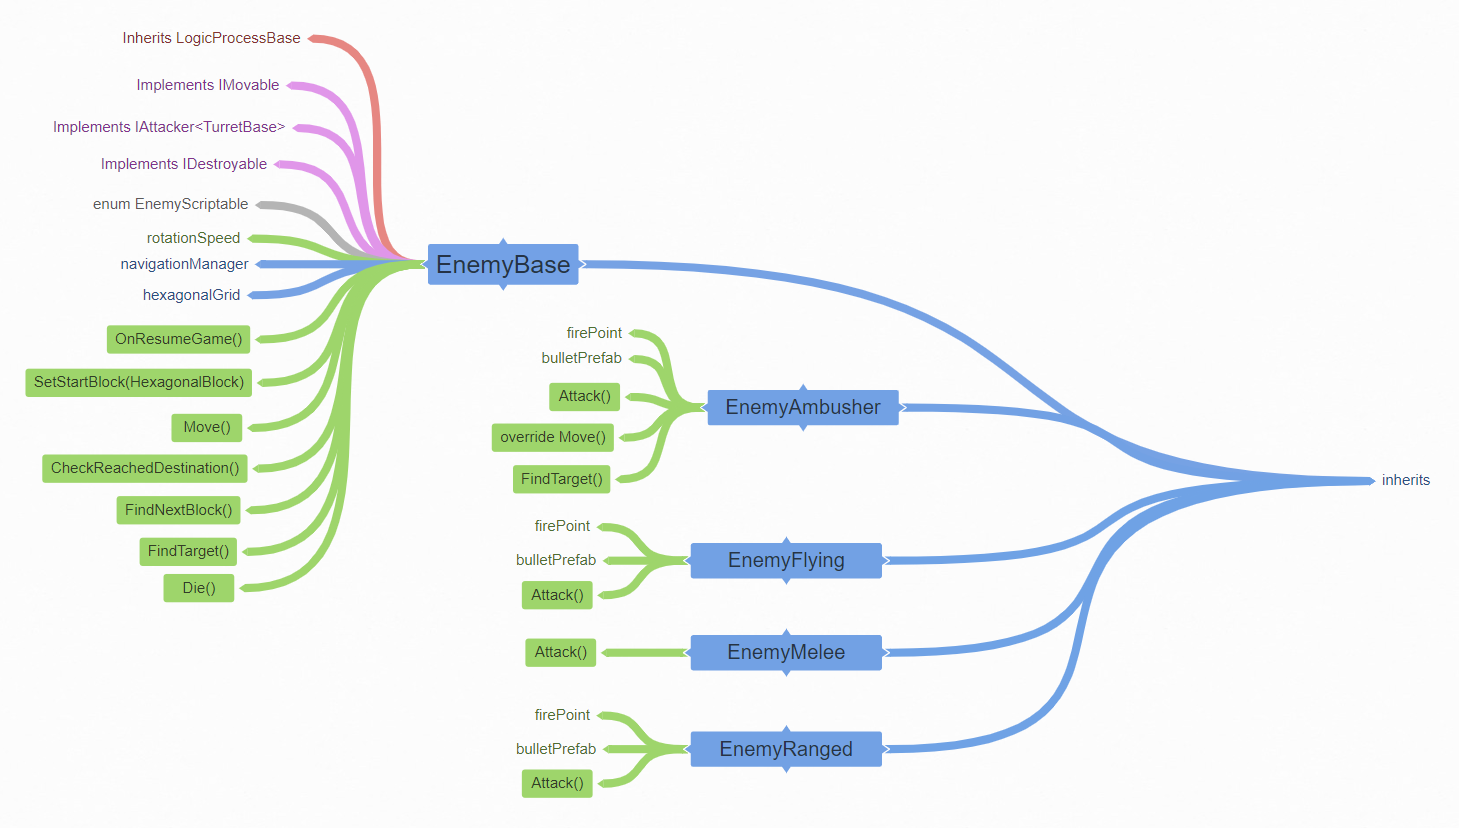
\includegraphics[width=1\textwidth]{EnemyHierarchy.png}
		\caption{Ierarhia inamicilor}
		\label{fig: enemyHierarchy}
	\end{figure}

	În fig: \ref{fig: enemyHierarchy} am definit într-un mod simplu și colorat modul în care trebuie structurată ierarhia inamicilor din joc.
	\newline
	
	Clasa EnemyBase este clasa părinte care definește modul principal în care inamicii trebuie să funcționeze. Această clasa implementează 3 interfețe utile, și anume IMovable, IDestroyable și IAttacker$\textless$TurretBase$\textgreater$. Precum am explicat și anterior, interfață IAttacker definește un șablon care specifică tipul de obiect pe care poate să îl atace, în cazul nostru, clasa TurretBase care va fi explicată în următoarea secțiune.
	\newline
	
	Această clasa face referire și la sistemul de navigare și la sistemul hărții hexagonale, și din acest motiv este nevoie să își facă inițializarea doar după ce aceste două sisteme și-au terminat inițializarea lor. În acest scop, putem să moștenim clasa LogicProcessBase, care a fost descrisă în capitolul \ref{section: initialization}.
	\newline
	
	Funcțiile implementate de această clasa sunt în mare parte funcțiile \newline moștenite după implementarile interfețelor descrie, cu câteva excepții referitoare la alte sisteme din joc. Un astfel de sistem este cel de a pune pe pauză jocul. Cand jocul este pus pe pauză, toate scripturile care se foloseau de timpul actual al jocului nu vor acționa în modul imediat de după ce reluăm jocul. Din acest motiv este nevoie să implementăm funcția OnResumeGame() care va fi apelata când se reia jocul, iar în această funcție trebuie să setam toți temporizatorii din script la valorile necesare.
	\newline
	
	Această clasa nu este suficientă pentru a definii toate tipurile de inamici, deoarece face dificilă diferențierea între inamici pentru anumite sisteme și anumiți inamici acționează diferit față de standard. Din acest motiv este necesar să definim o serie de clase pentru fiecare inamic în parte, care să moștenească această clasa de baza, și care să își adauge propia lor logică la standardul definit de EnemyBase.
	\newline
	
	\textbf{EnemyAmbusher} nu se folosește de sistemul de navigare. Este inamicul bombardier, care zboară prin aer direct către baza jucătorului. Când ajunge în contact cu această, lansează bombe care provoacă multe pagube, după care își continuă drumul, părăsind scena de lupa. Din acest motiv metodele Move() și FindTarget() trebuie să fie suprascrise.
	\newline
	
	\textbf{EnemyFlying} și \textbf{EnemyRanged} sunt inamici care urmează în totalitate logica definită de EnemyBase. Singura excepție la aceste două clase este că anumite turnuri vor face diferențiere între ele. O parte din turnuri pot să atace doar inamicii de sol (EnemyRanged și EnemyMelee) iar alte turnuri pot să atace doar inamicii zburători (EnemyFlying și EnemyAmbusher).
	\newline
	
	\textbf{EnemyMelee} este un inamic care poate să atace alte turnuri doar când a ajuns lângă acestea. Din acest motiv metoda lui de atac trebuie să fie suprascrisa puțin.
	
	
	
	
	
	\subsubsection{Ierarhia turnurilor defensive}
	\label{section: turretHierachy}
	
	Ierarhia turnurilor este puțin mai complexă și va fi descrisă pe bucăți.
	
	\ \\
	\textbf{TurretBase}
	
	Urmând aceeași logică ca la inamici, am definit o clasa de baza pentru modul în care trebuie să acționeze un turn defensiv. Acesta implementează două interfețe: IDestroyable și IAttacker$\textless$EnemyBase$\textgreater$. Șablonul de la IAttacker definește faptul că un turn defensiv poate să atace obiecte de tipul EnemyBase, care este clasa din care moștenesc toți inamicii jocului.
	\newline
	
	TurretBase are și ea nevoie de o initializare controlată și din acest motiv trebuie să moștenească clasa LogicProcessBase. TurretBase definește proprietățile turnurilor, cum ar fi viața, puterea de atac, etc. Pe lângă asta, majoritatea turnurilor pot fi îmbunatatine, proprietățile crescând exponențial când acest lucru se întâmplă. Din acest motiv a fost nevoie să creez fișiere configurabile care definesc valori pt proprietățile turnurilor. Această clasa deține o instanța a unui astfel de fișier, și definește o funcție "SetLevelProp(int level)" care citește fișierul configurabil și setează toate proprietățile în funcție de acesta. Pe lângă asta, când turnurile sunt îmbunătățite, le schimbă modelul 3D pentru a avea o schimbare vizuală.
	\newline
	
	Clasa definește și alte metode care au fost abordate în capitolele anterioare, precum: Die(), OnResumeGame(), Init(), etc. Funcția DrawRange() afișează/ascunde raza de atac a turnului, rază care a fost construită într-un shader special definit în Shader Graph.
	
	\ \\
	\textbf{PlayerBase}
	
	PlayerBase este o clasa care moștenește TurretBase, și reprezintă baza de operații a jucătorului. Aceasta implementează o parte din acțiunile definite în interfețe, precum: Attack(), FindTarget(), etc.
	\newline
	
	Pe lângă asta, când baza jucătorului rămâne fără viață și este distrusă, jocul trebuie să se termine. Acest lucru poate fi realizat foarte ușor prin suprascrierea metodei Die(). Când baza rămâne fără viață, înștiințează managerul jocului, iar pe urmă acesta își pornește procesul de încheiere al nivelului. Mai multe detalii vor fi discutate în capitolul \ref{section: gameState}.
	
	\ \\
	\textbf{BuildableTurret}
	
	BuildableTurret este clasa care moștenește TurretBase și definește \newline funcționalitățile pentru toate turnurile care pot fi construite pe harta de joc. Această clasa implementează IRecoverable, care definește modul în care turnurile pot să își refacă viață. De îndată ce turnul a fost lovit de un inamic, se calculează un cost necesar pentru a readuce turnul la viață maximă. În caz că jucătorul are suficienți bani și dorește să refacă turnul, acesta va începe procesul refacere. Pe parcursul câtorva secunde, se va reface treptat pentru viață lipsa în momentul începerii acestui proces. În acest timp turnul nu poate să atace inamicii, dar poate să fie lovit în continuare de aceștia, deci nu este garantat că va revenii la viață maximă după terminarea procesului.
	\newline
	
	O altă funcționalitate majoră a turnurilor este opțiunea de a îmbunatatii turnurile. Când utilizatorul selectează un turn, se caută în fișierul configurabil costul necesar pentru a îmbunătății turnul la nivelul următor, în caz că nu a ajuns încă la nivelul maxim. În caz că jucătorul are suficienți bani se apelează metoda Upgrade(), care verifică dacă s-a ajuns la nivelul maxim și dacă nu, dezactiveaza toate stările defavorabile ale turnului (cum ar fi raza), crește nivelul și apelează metoda SetLevelProp() pentru a citi din nou fișierul de configurație și actualiza starea turnului în funcție de acesta.
	\newline
	
	Turnul poate fi vantut de jucător în caz că este în criză de bani sau vrea să mute turnul în altă locație. În acest caz se calculează banii pe care îi primește jucătorul, se dezaciveaza toate stările și funcționalitățile turnului și se distrug referințele specifice. Tote acestea se întâmplă în metoda SellTurret() implementată în această clasa.
	\newline
	
	Ultima funcționalitate adăugată de această clasa este cea de a permite turnului să fie controlat de comandantul jocului. Această funcționalitate va fi descria în detaliu în secțiunea \ref{section: commander} 
	
	\ \\
	\textbf{Turnurile specifice}
	
	Cel mai jos nivel din ierarhie presupune definirea claselor specifice pentru fiecare tip de turn în parte, fiecare dintre acestea moștenind clasa BuildableTurret și adăugând/modificând logica stabilită până în acest punct în funcție de caz.
	
	\begin{itemize}
		\item \textbf{TurretElectricFence}. Este turnul care are viață foarte mare dar rază de atac foarte mică. Poate să atace doar inamicii de lupta apropiată și acționează drept un zid care păzește toate celelalte turnuri de atacurile inamicilor. Acest turn modifică funcționalitatea prin care se găsește ce inamic trebuie să atace și modul în care atacă inamicul.
		\item \textbf{TurretExcavator}. Acest turn este cel mai diferit de normă, în sensul în care nu poate atacă deloc inamicii. Este un turn care la un anumit interval de timp farmează resurse, pe care le convertește la bani de joc. Din acest motiv a fost nevoie să scape complet de căutarea inamicilor, iar metoda de atac a fost suprascrisă în funcționalitatea de farmare de bani.
		\item \textbf{TurretFlamethrower}. De îndată ce un inamic intră în rază acestui turn, lansează flăcări violente în direcția inamicului, flăcări care rănesc toți inamicii care stau în ele. Turnul prioritizează inamicii de atac de aproape, dar în cazul în care nu există astfel de inamici, atacă inamicii de la distanță. Nu poate să atace inamicii zburători sau cei bombardieri.
		\item \textbf{TurretMachineGun}. Este turnul universal care poate să atace toți inamicii jocului. Acesta lansează gloanțe foarte rapid către inamici, dar gloanțele individual nu provoacă foarte multe daune. Fiecare nivel presupune o viteză de atac mai mare.
		\item \textbf{TurretLaser}. Acest turn atacă inamicii cu un laser foarte puternic care distruge compoziția moleculară a inamicului în fiecare clipă în care aceștia sunt în raza turnului. Poate ataca inimacii de atac apropiat și cei de la distanță, dar îi prioritizează pe cei de la distanță. Nu poate ataca inamicii zburători sau pe cei bombardieri.
		\item \textbf{TurretVulkan}. Este turnul special împotriva inamicilor zburători și a celor bombardieri. Nu poate ataca inamicii de sol, dar în schimb lansează rachete către cei zburători, rachete care explodează când ajung în contact cu aceștia.
	\end{itemize}
	
	
	
	
	
	\subsubsection{Comandantul}
	\label{section: commander}
	
	Comandantul este un caracter special care poate fi mișcat oriunde dorim pe hartă și care atacă inamicii din raza lui de atac, cât timp nu se deplasează către o nouă locație.
	\newline
	
	În acest scop, clasa Commander implementează interfețele IMovable și IAttacker$\textless$EnemyBase$\textgreater$. Comandantul nu poate să fie distrus și din acest motiv nu este necesară implementarea interfeței IDestroyable.
	\newline
	
	Comandantul are și el un fișier de configurare care specifică statusurile lui, cum ar fi viața, viteza de mișcare, puterea de atac, etc. Pentru a se putea deplasa pe hartă, are nevoie să facă referire la sistemul de navigare și la cel al hărții de joc. Din acest motiv este necesar să moștenească LogicProcessBase, ca să își execute initializarea doar după ce celelalte sisteme au reușit să și-o termine pe a lor.
	\newline
	
	Majoritatea funcțiilor sunt similare cu cele ale turnurilor (Attack,\newline DrawRange, FindTarget, etc.) așa că nu vor fi reluate aici. 
	\newline
	
	Pe lângă aceste funcționalități, comandantul poate să intre în turnuri și să le controleze, mărindu-le astfel productivitatea. Când acesta intră în turnuri, le mărește raza, viteza, puterea de atac și în cazul excavatorului de resurse, crește banii primiți la fiecare livrare de resurse. Ca să poată intra în turnuri, trebuie să se deplaseze către acel turn la comanda jucătorului, iar când turnul este distrus/vândut, acesta iese din turn și se mișcă către cel mai apropiat nod din graful hărții de joc care nu este deja ocupat. Comandantul poate să iasă din turn și fără ca acesta să fie dsitrus, dar acest lucru se întâmplă numai la comanda jucătorului.
	
	
	
	
	
	\subsubsection{Punerea pe pauză a jocului}
	
	Jucătorul are la dispoziție opțiunea de a pune pe pauză jocul. Unity pune la dispoziție mai multe moduri de a pune pe pauză jocul. Unul din aceste moduri este de a modifica o variabilă din clasa globală Time, și anume Time.timeScale. Această variabilă are în mod normal valoarea 1, dar dacă o modificăm, toate sistemele jocului vor rula la o altă viteză. Dacă îi setăm o valoare de 0.5, majoritatea sistemelor vor încetinii (animații, sisteme de particule, rata de apelare a metodelor update, etc.). În caz că setăm această variabilă la 0, toate sistemele care sunt depentende de timp se vor opri din a funcționa până când se schimbă această variabilă. 
	\newline
	
	Este o metodă valida de a crea un sistem care să pună pe pauză jocul, dar deoarece oprește toate funcțiile update din a mai fi apelate și deoarece nu putem controla ce sisteme sunt oprite, nu este o metodă folosită foarte des. Un motiv principal pentru care nu este de recomandată această soluție este pentru că va opri inclusiv sunetele din joc, fapt ce nu este de dorit în cele mai multe cazuri.
	\newline
	
	O altă metodă de a implementa un sistem de pauză, este să avem un script care ține referințe către toate celelalte script-uri din scenă și care, în momentul în care jucătorul pune pe pauză jocul, oprește scripturile dorite din a mai fi executate. Unity are o clasa specială numită MonoBehaviour, care ne dă toate funcțiile discutate anterior (Start, Update, Coroutine, OnTriggerEnter, etc.) și multe alte proprietăți utile. Toate scripturile care moștenesc această clasa pot fi puse pe obiecte 3D din scenă, iar scripturile care nu implementează clasa MonoBehaviour nu pot fi puse pe obiecte din scenă. Acestea din urmă vor fi rulate numai când creăm obiecte de tipul acelor clase, sau în cazul claselor statice, când apelăm metode din ele. Clasele care moștenesc MonoBehaviour și care sunt puse pe obiecte 3D din scenă au o bifa lângă numele scriptului. În caz că bifa este dezactivată, scriptul nu va rula, iar această bifa poate fi setată și direct din cod, atâta timp cât avem referință la acest script. 
	\newline
	
	Revenind la ideea principala, script-ul care definește sistemul de pauză ar avea referințe la toate scripturile din scenă și decide pe care dintre acestea să le dezactiveze și pe care să le lase active în clipa în care jocul se pune pe pauză. Acest sistem nu presupune o implementare foarte frumoasă, deoarece în scene diferite putem avea scripturi diferite, iar acest lucru ne-ar determina să scriem mai multe scripturi de sistem de pauză, câte unul pentru fiecare scenă diferită în parte. Pe lângă asta, obținerea tuturor referințelor către scripturile din scenă este un proces greu de automatizat. Unity oferă câteva metode pentru găsirea scripturilor din scenă (FindObjectByType$\textless$type$\textgreater$(), FindObjectsByType$\textless$type$\textgreater$(), FindObjectByName$\textless$type$\textgreater$()), dar acestea nu pot găsi scripturile care sunt dezactivate. Alternativa ar fi să definim o lista sau variabile publice în care să punem scripturile dorite, dar acest proces presupune o pierdere de timp pentru programator și poate produce erori foarte ușor în caz că acesta uită să adauge scriptul în lista specifică.
	\newline
	
	Varianta pe care am implementat-o în cele din urmă este de a defini un script care pune pe pauză jocul și care are o serie de proprietăți care pot fi accesate de alte scripturi. Celelalte scripturi din scenă, în funcție de aceste proprietăți își vor modifică stările/sistemele în clipa în care jocul este pus pe pauză sau se reia. Această clasa am denumit-o GamePauseManager iar structura acesteia o vom explora în continuare.
	\newline
	
	GamePauseManager definește un Singleton, care este un concept de programare introdus în C\#. Singleton în Unity funcționează pe principiul că există o singură instanță a clasei în scenă, și din acest motiv, orice script poate face referire cu ușurință la această clasa, fără să mai fie nevoie să definim variabile publice și să dăm tragem scriptul în acele variabile publice. Singleton este menit pentru sistemele majore ale jocurilor/aplicațiilor, sisteme care au o singură instanța în scenă și care influențează o mare parte din scripturi. 
	\newline
	
	În Unity ca să definim un Singleton, în clasa dorită, definim o variabilă statică care are drept tip clasa din care face parte (de cele mai multe ori variabilă este numită instance). În metoda de Awake verificăm dacă acest instance este null, și dacă este, atunci setăm variabilă instance să fie egală cu pointer-ul this al clasei respective. Acest lucru setează variabilă statică să fie egală cu prima instanța a scriptului din scenă, astfel putem accesa scriptul direct din tipul clasei, fără a fi necesară căutarea acestuia (FindObjectOfType$\textless$type$\textgreater$()) sau crearea unei noi instanțe. 
	\newline
	
	În caz că nu extista o instanță a clasei în scenă, GamePauseManager.instance va rămâne null, ceea ce poate produce erori, motiv pentru care trebuie să ne asigurăm că adăugăm o instanța a clasei în fiecare scenă. Tot în metoda Awake, trebuie să verificăm și dacă instance este diferit de null, caz care se întâmplă când avem mai mult de o singură instanța a scriptului în scenă. Acest caz poate produce erori, motiv pentru care trebuie afișat un warning și distrusă instanța respectivă a scriptului (se șterg doar intantele scripturilor duplicate până în punctul în care rămânem cu o singură instanță a scriptului în scenă).
	\newline
	
	Pe lângă asta, scriptul definește câteva proprietăți publice care pot fi accesate direct de alte scripturi datorită singletonului implementat. Aceste proprietăți sunt următoarele:
	
	\begin{itemize}
		\item GamePaused boolean privat care specifică dacă în clipa curentă jocul este pus pe pauză sau nu, și care are implementat doar un getter ca să nu poată fi modificat de alte scripturi.
		\item PausedTime float privat care reprezintă cât timp a fost pus pe pauză jocul. Este util pentru reactualiza temporizatorii sistemelor. De asemenea, are doar un getter implementat pentru a nu permite altor scripturi să modifice proprietatea.
		\item PauseStartTime float privat care reprezintă timpul la care a fost pus pe pauză jocul. Este util pentru scripturile care se folosesc de Coroutine ca să își poată calcula corect timpul care trebuie așteptat.
		\item EventOnPauseGame este un delegate definit special pentru a înștiința alte scripturi când jocul este pus pe pauză. Toate scripturile care doresc, se pot abona la acest eveniment, iar în clipă în care este pus pe pauză jocul își pot opri/modifică sistemele care rulează
		\item EventOnResumeGame este de asemenea un delegate definit pentru a înștiința scripturile când jocul se reia. Scripturile care doresc se pot abona la acest eveniment pentru a își reactualiza stările și a repornii sistemele în clipa în care jocul revine la normal.
	\end{itemize}
	
	Clasa are și câteva metode definite pentru a procesa interacțiunea utilizatorului cu UI-ul, deoarece UI-ul de pauză de joc rămâne neschimbat între scenele jocului. Când jocul este pus pe pauză, pe ecran apare un mesaj care înștiințează jucătorul, și mai apar 2 butoane: "Exit Level" și "Quit Game". În caz că apasă pe vreunul din ele, este întrebat dacă este sigur de alegerea dorită și în caz că răspunde afirmativ, este scos din nivel/joc în funcție de caz. Pentru a relua jocul, trebuie să apese din nou pe butonul de pauză, meniul va dispărea și jocul se va relua.
	
	
	
	
	
	\subsubsection{Valul de inamici}
	\label{section: enemyWave}
	
	Pe parcursul nivelului, inamicii vin în mai multe valuri. Un val de inamici constituie o serie de inamicii diferiți sau identici care apar într-o ordine prestabilită sau la întâmplare. Metoda de implementare care mi s-a părut cea mai ușoară a fost să definesc fișiere de configurare care conțin structura valurilor de inamici. Aceste fișiere configurabile le-am definit folosind un concept specific Unity, și anume ScriptableObject. Aceste obiecte sunt instanțe ale unei clase a cărei structuri o putem defini. Obiectele sunt obiecte globale care pot fi modificate direct din editor și care permit accesarea valorilor din interiorul obiectului cu ușurință, de către scripturile care au nevoie de această informație. Utilizând acest concept, am creat un Scriptable Object numit WaveScriptable, care conține următoarele date:
	
	\begin{itemize}
		\item SpawnRandomly este un boolean care specifică dacă inamicii apar în ordinea prestabilită sau la întâmplare.
		\item ID-ul punctului de pe harta din care vor apărea.
		\item O lista de perechi de câte două valori. Prima valoare din pereche reprezintă inamicul care va apărea pe harta, iar a două valoare reprezintă câți inamici de acest tip vor apărea unul după altul, în caz că spawnRandomly este fals, sau aleatoriu în caz contrar.
	\end{itemize}
	
	Folosind această structură, putem crea o multitudine de valuri de inamici, numărul de inamici și ordinea acestora fiind diferită.
	
	
	
	
	
	\subsubsection{Stagiile jocului}
	\label{section: stageScriptable}
	
	Valurile de inamici nu reprezintă suficientă informație pentru a acoperii un nivel, deoarece majoritatea nivelelor nu vor conține un singur val. În acest scop am creat o structura similară cu cea a valului de inamici, dar la un nivel mai înalt.
	\newline
	
	StageScriptable este un Scriptable Object care definește care valuri de inamici apar la stagiul curent, și multe alte proprietăți pentru a face nivelele cât mai variate.
	
	\begin{itemize}
		\item StageName reprezintă numele pe care îl definim noi pentru stagiul respeciv. Este folosit de multe sisteme, și anume: încărcarea configurării hărții de joc pe baza căutării unui fișier cu numele specificat de stageName, crearea UI-ul dinamic în scena în care selectăm nivelul pe care dorim să îl jucăm, lucru care va fi discutat în capitolul \ref{section: levelSelection}
		\item O listă de tipul WaveScriptable, în care putem pune toate obiectele create pentru valurile de inamici. Astfel putem crea o serie de nivele variate. O parte din valurile de inamici se pot repeta* între stagii, dar stagiile trebuie să fie unice.
		\item IsBossStage este un boolean care ne ajută să identificăm dacă suntem în modul co-op sau nu. Mai multe detalii vor fi discutate în capitolul \ref{section: coop} 
		\item Banii pe care îi primim dacă reușim să câștigăm nivelul. Banii sunt folosiți pnetru sistemul de îmbunătățiri permanente, discutat în capitolul \ref{section: permanentUpgrade}
		\item Numărul de stele câștigate până acum la stagiul respectiv. Acest concept va fi discutat în capitolul următor.
	\end{itemize}
	
	
	
	
	
	\subsubsection{Controlul jocului}
	\label{section: gameState}
	
	În punctul acesta am reușit să creăm fișiere configurabile pentru o multitudine de nivele diferite, dar este necesar să scriem un sistem care poate citi aceste fișiere configurabile și care controlează ordintea în care apar inamicii și stările jocului.
	\newline
	
	WaveManager este script-ul care citește propriu-zis fișierul configurabil (StageScriptable) și care controlează modul în care apar inamicii pe hartă. Acesta definește o corutină care primește ca parametru fișierul configurabil al valului de inamici (preluat din lista de valuri din fișierul stagiului). Corutină ne ajută să așteptăm o periada anume între aparițiile inamicilor pe hartă. La începutul corutinei, toți inamicii sunt adăugați într-o lista în ordinea în care sunt specificați în fișierul configurabil. În caz că spawnRandomly este adevărat, reordonăm lista într-un mod aleator folosindu-ne de metoda Shuffle(). Pe urmă, pornim un loop peste fiecare element din lista. La fiecare element creăm un obiect de tipul inamicului respectiv, îl poziționăm pe hartă în locul dorit, pornim procesul de inițializare al acestuia și așteptăm un anumit număr de secunde până la următoarea interatie.
	\newline
	
	După ce toți inamicii au fost astfel instanțiați, se așteaptă o perioada de 30 de secunde, după care se trece la valul următor. În acest timp jucătorul este liber să își refacă sau îmbunătățească turnurile, sau, în caz că se simte încrezător, poate să sară peste această perioada, primind contravaloarea timpului în bani de joc. După ce toate valurile au fost instantiate, controlul este preluat de scriptul BattleStageStateManager, despre care vom discuta in continuare.
	\newline
	
	BattleStageStateManager este scriptul care controlează finalul nivelului, final obținut prin distrugerea bazei jucătorului sau prin omorârea tuturor inamicilor. În metoda Die() din clasa PlayerBase, discutată în capitolul \ref{section: turretHierachy}, apelăm metodă GameOver() din clasa BattleStageManager. Această metodă afișează pe ecran meniul de pierdere a jocului și pune pe pauză jocul pentru a nu permite anumitor sisteme să nu mai funcționeze corespunzător (din cauza lipsei bazei jucătorului) și a nu permite inamicilor să se deplaseze de bună voie pe hartă. La acest meniu de pierdere a jocului afișăm jucătorului că a câștigat 0 stele, afișăm banii câștigați în urma distrugerii inamicilor până în punctul actual și așteptăm ca acesta să apese ecranul, moment în care este trimis la scena de selectare a nivelelor, discutată în următorul capitol.
	\newline
	
	Celălalt mod în care jocul poate fi terminat este după instanțierea tuturor valurilor de inamici. După ce toate valurile au fost instanțiate, WaveManager înștiințează BattleStageStateManager de acest lucru, moment în care acesta verifică o dată la câteva cadre de joc dacă mai sunt inamici în viață pe hartă. În clipa în care nu mai sunt inamici pe hartă, se afișează meniul de câștigare a jocului și se așteaptă ca jucătorul să apese ecranul, moment în care este trimis la scena de selectare a nivelelor, discutată în următorul capitol. Pe meniul de câștigare a jocului se afișează banii și numărul de stele câștigate. 
	\newline
	
	Stelele reprezintă cât de bine s-a descurcat jucătorul în a își apară baza de operațiuni pe parcursul nivelul. În caz că aceasta are mai mult de 90\% din viața maximă, jucătorul s-a descurcat excelent și primește 3 stele. În caz că baza are peste 40\%, atunci jucătorul s-a descurcat la un nivel acceptabil și primește 2 stele. În caz că baza are sub 40\% atunci a reușit să supraviețuiască nivelul la limita și primește o singură stea drept consecință. Stelele influențează numărul de bani primiți la terminarea nivelului. Fiecare stea câștigată pentru prima dată la nivelul respectiv aduce o recompensă monetară pentru jucător, recompensă care poate fi folosită să își îmbunătățească turnurile. 
	\newline
	
	În caz că jucătorul se blochează la un moment dat și nu paote trece de un anumit nivel, este recomandat să se întoarcă la nivelele anterioare, să câștige 3 stele la toate aceste nivele, să își îmbunătățească turnurile și să se întoarcă mai puternic că niciodată la nivelul care îi provoca dificultăți.
	
	
	
	
	
	\subsection{Selectarea nivelelor}
	\label{section: levelSelection}
	
	\subsubsection{Structura meniului}
	
	La pornirea aplicației putem vedea un meniu cu mai multe opțiuni. Dacă utilizatorul apasă pe butonul "Start Game", va fi dus la un meniu din care poate să selecteze nivelul pe care dorește să îl joace.
	
	În partea stânga putem vedea un buton care ne duce înapoi la pagina principală. Pe lângă aceasta, în colțul din dreapta sus avem un alt buton intitulat "Shop" care ne va duce la magazinul de îmbunătățiri permanente, care va fi discutat în capitolul \ref{section: permanentUpgrade}. În colțul din dreapta jos putem observa banii adunați de jucător până în punctul curent. La începutul jocului are 0 bani, iar pe măsură ce câștigă nivele și stele la nivelele respective, numărul de bani va crește.
	\newline
	
	Esența acestui meniu este panoul din centrul ecranului. În partea dreapta a panoului putem observa o lista de nivele. Fiecare nivel are un titlu anume și 3 stele negre. După ce câștigăm un nivel, stelele câștigate la nivelul respectiv vor apărea în locul stelelor negre pentru a ne înștiința progresul făcut la nivelul respectiv.
	\newline
	
	Dacă apăsăm pe unul din nivele, meniul din stânga va fi umplut cu informații. Prima informație pe care o putem vedea este că apare o imagine cu harta de joc pe care va lua loc nivelul. Sub această imagine sunt scrise informații legate de nivelul respectiv:
	
	\begin{itemize}
		\item Numele stagiului selectat.
		\item Inamicii întâlniți și numărul fiecărui tip de inamic.
		\item Banii primiți în cazul câștigării nivelului. Aceștia sunt banii de baza, pe care îi va primi jucătorul indiferent de numărul de stele câștigate. Stelele aduc o contravaloare în plus față de această suma, contravaloare plătită numai în clipa în care steaua respectivă este câștigată pentru prima dată. Dacă prima dată când jucăm un nivel câștigăm 2 stele și a două oară când jucăm același nivel câștigăm tot 2 stele, nu vom primi bani extra pe cele 2 stele câștigate. În caz că a două oară când jucăm nivelul primim 3 stele, vom primii contravaloarea unei singure stele, deoarece doar aceasta este steaua care a fost câștigată pentru prima dată.
	\end{itemize}
	
	Putem să mai observăm și un buton intitulat "Start Stage", care va începe nivelul respectiv. Acest buton salvează nivelul selectat într-un obiect indestructibil între scene, concept care va fi discutat în capitolul \ref{section: dataBetweenScenes}, după care încarcă scena de lupta. Odată ajuns în scena de lupta se preiau datele nivelului încărcat in obiectul indestructibil, se generează automat harta de joc, se inițializează toate celelalte scripturi necesare și se așteaptă ca jucătorul să apese pe butonul de începere a jocului.
	\newline
	
	\subsubsection{Generarea dinamică a meniului}
	
	Acest meniu este generat automat la începutul acestei scene, în funcție de fișierele configurabile ale stagiilor de luptă create (StageScriptable).
	\newline
	
	Pentru generarea dinamică a meniului a fost necesară crearea unui prefab ajutător: StageUIBlock. Acest prefab conține butonul pe care poate apasa jucătorul și 6 stele: 3 dintre stele sunt negre, iar celelalte 3 stele sunt galbene și sunt suprapuse cu cele negre. Când câștigăm un nivel tot ce trebuie să facem este să activăm aceste stele galbene, urmând ca ele să fie randate în fața celor negre. Acest prefab conține și un script care controlează ce nume este afișat pe buton și care stele galbene trebuie să fie activate. Acest lucru se întâmplă în metoda InitializeBlock(StageScriptable stage), care inițializează toate proprietățile prefab-ului în funcție de nivelul pe care îl reprezintă. Acest script generează și descrierea nivelului, descriere care conține: numele nivelului, inamicii, numărul de inamici întâlniți din fiecare tip și banii primiți în urma câștigării nivelului.
	\newline
	
	Pe lângă acest prefab, a fost necesară scrierea unui script care să creeze, poziționeze și inițializeze clone ale acestui prefab, în funcție de fișierele de configurare care au fost definite pentru joc. Scriptul se numește StageUISpawner.
	\newline
	
	Ultima clasa relevantă din această scenă este StageSelectionManagement, care controlează obiectele StageUIBlock selectate și informația afișată de pe acestea. În momentul apăsării unui buton de pe obiectul StageUIBlock, se înștiințează managerul că obiectul respectiv a fost afișat, urmând ca managerul să preia datele necesare de pe obiect și să le afișeze corespunzător pe interfața utilizatorului. Acesta este responsabil și prentru schimbarea între scene.
	
	
	
	
	
	\subsubsection{Transmisia datelor între scene}
	\label{section: dataBetweenScenes}
	
	Obiectul amintit mai sus se numește SceneDataRetainer. În Unity în mod normal, când schimbăm între scene, toate obiectele din scenă curentă vor fi distruse și vor fi înlocuite cu cele din scena pe care dorim să o încărcăm. Acest lucru include și scripturile de pe obiecte, fapt care face transmisia de date între scene să fie dificilă. Există totuși câteva variante prin care pot fi transmise datele între scene, variante care vor fi discutate în continuare.
	\newline
	
	Una dintre variantele valide și foarte des folosite de a transmite datele între scene este să salvăm datele pe disk înainte să încărcăm scena, iar după ce am încărcat scena să citim acel fișier, să procesăm datele din acesta și să inițializăm scripturile dorite în funcție de datele procesate. Unity a definit și o clasa specială pentru acest mod de lucru și anume PlayerPrefs. În clasa PlayerPrefs putem salva orice date dorim și putem să le accesăm din alte scene cu ușurință, prin simpla apelare a câtorva metode simple. Clasa PlayerPrefs în spate funcționează tot prin salvarea și citirea anumitor fișiere pe disk, iar metodele expuse de clasă apelează acele funcționalități specifice. Această metodă este utilă când vrem să salvăm date simple între scene, dar nu și când avem obiecte complexe, deoarece de cele mai multe ori ar trebuii să creăm din nou obiectul respectiv după ce îl citim din fișier. O altă limitare este că nu pot fi stocate date și fișiere foarte mari între scene, deoarece citirile și scrierile pe disk ar dura foarte mult timp, fapt ce ar întrerupe jocul. Ultima limitare relevantă este că, pe anumite dispozitive, nu avem acces să citim/scriem oriunde dorim noi, fapt ce ar determina PlayerPrefs să nu funcționeze corespuzator pe acele dispozitive. Mai multe lucruri vor fi discutate despre acest subiect în capitolul \ref{section: androidSave}
	\newline
	
	Cealaltă metodă de lucru este cea pe care am ales să o folosesc, și anume folosirea unui obiect nemuritor. Pentru a defini un astfel de obiect, în metoda Awake sau Start din scriptul repsectiv, trebuie să apelăm metoda DontDestroyOnLoad() și să îi dăm ca parametru obiectul pe care se află scriptul respectiv. Acest lucru va înștiința Unity-ul că obiectul respectiv nu trebuie șters la încărcarea între scene. Astfel transmisia de date între scene devine foarte ușoară, trebuie să definim variabile publice sau private cu geteri și seteri pentru a permite salvarea și citirea corectă a datelor. SceneDataRetainer de asemenea are un Singleton implementat pentru a permite accesarea datelor între scene cu ușurință. În această clasa am ales să salvez următoarele date:
	
	\begin{itemize}
		\item SelectedStage este o variabilă de tipul StageScriptable care are definit getteri și setteri. În această variabilă salvăm nivelul selectat de jucător, pentru a putea inițializa scena de lupta în momentul incarcarii acesteia.
		\item PermanentUpgrades este o variabilă de tipul TurretPermanentUpgrades[] care are de asemenea definiți getteri și setteri. Această variabilă reține coeficientii de îmbunătățire a turnurilor, în urmă achiziționării lor din magazinul de îmbunătățiri permanente. Mai multe detalii în capitolul \ref{section: permanentUpgrade}.
		\item SelectedBossDifficulty este o variabilă de tipul BossScriptableObject. Această variabilă reține proprietățile monstrului din scena co-op, care va fi discutată în capitolul \ref{section: coop}.
	\end{itemize}
	
	Acest script generează totuși o problema. În caz că punem scriptul acesta direct pe un obiect din scenă, în prima iteratie va funcționa corespunzător. Vom putea încarcă un nivel, să jucăm normal prin acel nivel, iar la finalul lui revenim la scena de selectare a nivelelor jocului. În acest punct vom avea 2 instanțe ale scriptului: unul din scripturi este cel nemuritor pe care l-am păstrat între scene, iar al doilea este cel nou creat când am încărcat scenă de selectare a nivelelor. Deoarece el era setat din start în scenă, de fiecare dată când reîncărcăm scenă, va fi creată o nouă instanța a scriptului. Acest lucru poate să strice sistemele existente, din acest motiv este necesară scrierii unui alt script.
	\newline
	
	SceneIndependentScriptsSpawner este un script care la începutul jocului verifică dacă avem scripturi nemuritoare în scenă. În caz că avem, atunci se distruge singur fără să mai facă nimic. În caz că nu avem scripturi nemuritoare, creează obiectele nemuritoare dorite, le inițializeaza, după care se distruge singur pentru a opri orice altă funcționalitate. Acest simplu script rezolva problema duplicarii de obiecte nemuritoare între scene.
	
	
	
	
	
	\subsection{Magazinul de îmbunătățiri permanente}
	\label{section: permanentUpgrade}
	
	\subsubsection{Structura meniului}
	
	Poate fi accesat din meniul selectării nivelului de joc. La acest meniu putem vedea în colțul din dreapta jos, banii pe care i-a adunat jucătorul până în clipă curentă. În stânga sus avem un buton care ne duce înapoi la meniul selectării nivelului de joc. În centrul ecranului putem vedea butoane cu numele turnurilor noastre. În caz că apăsăm pe unul din butoane, în dreapta acestora va apărea o nouă interfață grafică.
	\newline
	
	Putem observa că au apărut 3 rânduri, fiecare rând continant o serie de informații:
	
	\begin{itemize}
		\item Numele proprietății care este îmbunătățită pentru turnul curent.
		\item Zece dreptunghiuri care pornesc de la mic la mare. Aceste blocuri vor fi umplute cu diverse culori pe măsură ce îmbunătățim proprietatea specifică a turnului selectat.
		\item Un buton de plus care cumpără un nivel nou pentru proprietatea respectivă. Nivelul maxim care poate fi cumpărat este 10.
		\item Sub butonul de plus apare costul cumpărării pentru îmbunătățirea respectivă. Acest cost se calculează infunctie de nivelul actual al jucătorului. În caz că nu are suficienți bani, textul este colorat cu roșu, și dacă apasă pe butonul de plus nu se va întâmpla nimic. La nivelul maxim, în loc de un cost, va apărea cuvântul "MAX" în acest loc.
	\end{itemize}
	
	Îmbunătățirile pentru fiecare tip de turn în parte sunt:
	
	\begin{itemize}
		\item Gardul electric: rată și putere de atac mărită, viață extra
		\item Excavatorul: rată și putere de atac mărită, viață extra
		\item Aruncătorul de flăcări: putere și rază de atac mărită, viață extra
		\item Mitralieră automată: rată, putere și rază de atac mărită
		\item Baza jucătorului: rată și putere de atac mărită, viață extra
		\item Laserul: putere și rază de atac mărită, viață extra
		\item Vulkan: rată, putere și rază de atac mărită
	\end{itemize}
	
	Toate aceste elemente au fost generate dinamic la încărcarea scenei, fapt pe care îl vom investiga în detaliu în cele ce urmează. Ca să putem discuta despre generarea dinamică a meniului, trebuie mai întâi să parcurgem cum este reprezentată o îmbunătățire permanentă și cum este folosită în alte scripturi.
	
	
	
	
	
	\subsubsection{Îmbunătățire permanentă}
	
	Îmbunătățirea permanentă este un simplu coeficient cu care sunt înmulțite toate propietatile turnurilor la începutul unui nivel de lupta. Totuși, pentru folosirea acestui coeficient a fost necesară folosirea mai multor informații, motiv pentru care am creat o clasa specială, PermanentUpgrade, care are următoarele proprietăți:
	
	\begin{itemize}
		\item UpgradeType este un enum care definește tipul îmbunătățirii. Acesta poate fi una din următoarele: viteză, putere, rază de atac și viață extra.
		\item Valori de minim și maxim între care se poate afla coeficientul îmbunătățirii respective. Acest lucru ne ajută să calculăm cu ușurință coeficientii respectivi la fiecare nivel al îmbunătățirii.
		\item Coeficientul propriu-zis cu care înmulțim proprietățile turnurilor.
		\item Costul de start pentru a cumpăra prima îmbunătățire.
		\item Un coeficient cu care este înmulțit prețul curent al îmbunătățirii, în momentul cumpărării acesteia. Rezultatul operației este salvat drept costul pentru următoarea îmbunătățire
		\item Nivelul curent al îmbunătățirii.
		\item Nivelul maxim la care poate fi dusă îmbunătățirea. Momentan a fost setat la 10.
	\end{itemize}
	
	Cu această clasa am reușit să definim cum ar trebuii să arate o îmbunătățire, dar un turn are 3 îmbunătățiri, iar de preferat ar fi să putem modifica cu ușurință aceste valori. Din acest motiv am creat o nouă clasa care moștenește ScriptableObject și care definește o serie de proprietăți:
	
	\begin{itemize}
		\item Tipul turnului la care se aplică îmbunătățirea.
		\item O lista de îmbunătățiri posibile pentru turnul respectiv. Lista conține elemente de tipul PermanentUpgrade, care a fost explicat mai sus.
		\item O metodă prin care putem obține coeficientul. Acesta primește ca și parametru tipul de îmbunătățire dorit. Funcția caută în lista de îmbunătățiri dacă există acea îmbunătățire dorită, și dacă există, atunci returnează coeficientul acesteia. În caz contrar returnează 1 pentru a nu modifică proprietățile turnurilor.
	\end{itemize}
	
	\subsubsection{Generarea dinamică a meniului}
	
	Pentru generarea dinamică a meniului am creat un prefab cu un buton și un text pe el, care reprezintă butoanele cu numele turnurilor. Aceste butoane vor fi generate automat folosind prefab-ul respectiv. Pe fiecare din aceste butoane se adaugă un delegate care va fi apelat în momentul apăsării pe buton. Acest delegate schimbă index-ul turnului selectat și actualizează informația de pe ecran în funcție de noul index.
	\newline
	
	O altă clasa folosită este UIUpgradeRow, care controlează afișarea și cumpărarea îmbunătățirii permanente (rândul din dreapta care apare în momentul selectării turnului pe care dorim să îl îmbunătățim). Acest script este activat și inițializat în momentul în care apăsăm pe unul din butoanele explicate anterior, moment în care activează dreptunghiurile de pe ecran în funcție de nivelul actual al îmbunătățirii. Pe lângă asta, calculează și costul cumpărării următorului nivel pt îmbunătățirea respectivă, afișează acest cost pe ecran, iar în cazul în care jucătorul nu are suficienți bani, colorează cu roșu acest cost. De asemenea, în momentul în care jucătorul cumpără o îmbunătățire, se apelează o metodă din această clasa, care calculează din nou costul proprietății, îl afișează pe ecran, și înștiințează managerul magazinului că jucătorul dorește să cumpere îmbunătățirea respectivă. În acea clipă, managerul magazinului scade banii pe care ii deține jucătorul, actualizează coeficientul și datele îmbunătățirii și pornește salvarea datelor, care va fi discutată în capitolul următor.
	\newline
	
	Deoarece există 3 îmbunătățiri pentru fiecare turn, UIUpgradeRow se va afla pe fiecare din cele 3 rânduri, diferența dintre ele fiind proprietatea pe care o monitorizează. Această proprietate este setată în momentul în care apăsăm pe butonul cu numele turnurilor, UI-ul modificandu-se în funcție de proprietățile turnului selectat. La fiecare îmbunătățire, datele sunt salvate automat și în memorie dar și pe disk, astfel nefiind posibilă pierderea datelor.
	
	
	
	
	
	\subsection{Salvarea datelor}
	
	Salvarea datelor este un concept întâlnit în toate jocurile existente, dar și în alte tipuri de aplicații. Orice joc are nevoie să salveze anumite date: date cu progresul jucătorului, date cu configurări ale jucătorului, date colectate de dezvoltatori pentru a își îmbunătății jocul/aplicația, etc. Deoarece este un concept atât de important și am dorit ca jucătorul să aibă parte de o experiență cât mai bună a trebuit să implementez un astfel de sistem și pentru joc.
	\newline
	
	Fișierele de configurare necesare pentru ca jocul să funcționeze corespunzător au fost discutate la fiecare capitol în parte unde erau necesare, motiv pentru care nu vor fi reluate aici.
	
	
	
	
	
	\subsubsection{Datele care trebuie salvate}
	
	În primul rând trebuie să discutăm despre ce date este necesar să fie salvate pentru ca jucătorul să poată continua de unde a rămas, în urmă întreruperii sesiunii de joc. În acest scop, am definit o clasa PlayerData a cărei structura definește tipurile de date care trebuie salvate pentru un anumit jucător. Clasa conține banii câștigați de jucător și o lista cu progresul acestuia la fiecare nivel al jocului. 
	\newline
	
	Informația progresului pentru fiecare nivel am organizat-o într-o clasa separată pentru a ușura modul de lucru. Clasa se numește StageSaveData și conține două proprietăți: numele nivelului, pentru a putea fi identificat cu ușurință, și numărul de stele câștigate la nivelul respectiv.
	\newline
	
	Pe lângă aceste date, pentru un anumit jucător salvăm și îmbunătățirile cumpărate de jucătorul respectiv. Îmbunătățirile au structura prezentată în capitolul \ref{section: permanentUpgrade}.
	
	
	
	
	
	\subsubsection{Salvarea automată}
	
	Salvarea propriuzisa este controlată de un script nemuritor, definit cu tipul PlayerDataSaver. Acest script este creeat și inițializat în același timp cu SceneDataRetainer, și are implementat și un singleton pentru a permite scripturilor din scenă să îl acceseze cu ușurință.
	\newline
	
	Scriptul are definit o metodă SaveData(), care preia toate datele utilizatorului, discutate mai sus și le convertește la o structura JSON, pentru a ușura procesarea datelor. După convertire, aplică o criptare simplistă peste aceste date, pentru a nu permite jucătorului să modifice datele după bunul lui plac. Metoda de criptare aplică un operator XOR între fiecare caracter din fișierele JSON și o cheie definită în program. Această operație face ca mesajul JSON să fie inteligibil pentru oameni. După ce a terminat criptarea datelor, salvează mesajele rezultate în 2 fișiere: primul fișier conține datele jucătorului (banii și progresul la fiecare nivel în parte), iar al doilea fiser conține îmbunătățirile cumpărate de acesta.
	\newline
	
	Deoarece salvăm datele pe disk, trebuie să avem definită și o metodă pentru a prelua aceste date. Metoda este denumită simplist: LoadData și, folosind tratarea de excepții, încearcă să citească și să proceseze datele de pe disk. Metoda este împărțită în două faze și aplică tratarea de excepții în fiecare dintre faze. 
	\newline
	
	Prima faza este cea de citire a datelor jucătorului (primul fișier salvat). În această situație, citește conținutul fișierului de pe disk, aplică din nou aceeași operație de criptare, care va readuce textul la starea lui inițială, urmând să îl convertească la un obiect de tipul PlayerData. Motivul principal pentru care am ales să folosesc formatul JSON, este pentru că există multe funcționalități deja implementate pentru serializare și deserializare de fișiere JSON. Serializarea presupune convertirea unui obiect din memorie la un string cu formatul specific JSON, pe când deserializarea presupune convertirea unui string în formatul JSON la un obiect în memorie. Aplicând procesul de deserializare pe string-ul rezultat în urmă decriptarii, obținem în memorie un obiect de tipul PlayerData.
	\newline
	
	Folosindu-ne de acest obiect, inițializăm toate celelalte date relevante din joc. În cazul în care fișierul lipsește sau este corupt, se resetează toate stările de joc la o stare de baza, în care jucătorul are progres la vreun nivel, nu deține bani în posesie și nu a cumpărat nici o îmbunătățire permanentă.
	\newline
	
	A două faza este cea de citire a îmbunătățirilor cumpărate de jucător. Acestea erau salvate într-un fișier separat, iar procesul este similar cu cel de mai sus. Citim fișierul de pe disk, îl decriptăm aplicând aceeași operație XOR cu aceeași cheie, deserializam obiectul, astfel obținând un obiect de tipul TurretPermanentUpgrades[], urmând să modificăm datele jocului în funcție de aceste date citite de pe disk.
	\newline
	
	La fel ca și în cazul primei faze, în caz că lipsește fișierul de pe disk, sau fișierul respectiv a fost corupt, jocul se resetează la starea lui inițială. Fișierul poate devenii corupt din o serie de motive:
	
	\begin{enumerate}
		\item Programatorul a schimbat cheia folosită pentru decriptare între rulări ale aplicăției.
		\item Jucătorul a găsit fișierele salvate pe disk și a încercat să le modifice.
		\item Jucătorul a închis aplicația brusc cât timp se afla în procesul de salvare a datelor, rezultând într-un fișier incomplet. Acest caz este puțin probabil, deoarece datele care sunt salvate sunt puține, și salvarea se face numai în momentul în care s-a terminat de procesat toate datele. Dacă salvarea pe disk se aplică treptat, atunci era cu mult mai probabilă coruperea fișierului.
	\end{enumerate}
	
	Cu ajutorul acestor operații, putem concepe cu ușurință un sistem de salvare automată, și anume: de fiecare dată când jucătorul modifică o parte din date (câștigă un nivel, cumpără o îmbunătățire), apelăm metoda SaveData din acest script, care va suprascrie datele jucătorului cu cele curente.
	
	
	
	
	\subsubsection{Locația fișierelor salvate pentru dispozitive diferite}
	\label{section: androidSave}
	
	Unity pune la dispoziție două metode utile pentru a controla locațiile în care se salvează datele, și anume:
	
	\begin{itemize}
		\item Application.streamingAssetsPath. Această proprietate returnează o locație din folderul jocului, în care sunt salvate toate resursele plasate în folderul StreamingAssets în editor.
		\item Application.persistentDataPath. Această proprietate returnează o locație în afara folderului jocului și diferă în funcție de platforma de pe care se rulează. Pe Windows, acest folder poate fi găsit de obicei în \newline AppData/LocalLow/$\textless$companyname$\textgreater$/$\textless$productname$\textgreater$. Pe android, de obicei se află la locația \newline
		/storage/emulated/0/Android/dată/$\textless$packagename$\textgreater$/files.
	\end{itemize}
	
	În cazul rulării aplicăției pe Windows, putem alege ambele variante, singura diferență este dacă dorim să păstrăm datele după ce ștergem jocul sau nu. În caz că nu vrem să păstrăm datele, trebuie să folosim Application.streamingAssetsPath, iar în caz că vrem să fie păstrate, trebuie să folosim Application.persistentDataPath.
	\newline
	
	Pe Android este o cu totul altă poveste. Toate fișierele jocului sunt compresate într-un singur fișier .apk, motiv din care nu putem scrie în acest fișier. Putem doar să aplicăm citiri, motiv pentru care, pe android trebuie să folosim Application.persistentDataPath, care ne dă o locație în care putem aplica și citiri și scrieri.
	\newline
	
	Din această cauză, am creat o clasă specială, FileManager, care controlează locațiile la care se aplică citiri și scrieri de fișiere. Acest script funcționează diferit în funcție de platforma pe care este rulat, datorită folosirii unor directive specifice, și are 2 metode definite: SetFileContents și GetFileContents. Ambele metode primesc ca și parametrii un boolean care definește dacă vrem să salvăm în streaming assets sau nu, în caz contrar se salvează la locația persistența. Al doilea parametru reprezintă string-ul pe care vrem să îl punem în fișier, iar ultimul parametru reprezintă numele fișierului în care salvăm sau din care citim conținutul.
	
	
	\subsection{Sistemul co-op}
	\label{section: coop}
	
	Pentru a putea diferenția jocul acesta față de alte jocuri pe acest stil din domeniu, am decis să implementez un mod co-op, în care joci un nivel dificil împreună cu un alt jucător. Momentan este implementat un singur nivel de acest tip, dar care are mai multe dificultăți care pot fi explorate. Pe lângă această, majoritatea functionalitatilor sunt deja scrise, motiv pentru care pot fi create cu o relativă ușurință și alte nivele de joc.
	\newline
	
	Sincronizarea a fost realizată cu ajutorul un framework numit Photon Engine, despre care vom vorbi în continuare.
	
	
	
	
	
	\subsubsection{Modul de lucru cu Photon Engine}
	
	Photon Engine este un framework dezvolat de Exit Games. Acest framework are mai multe pachete care pot fi achiziționate. O parte dintre acestea sunt gratis, iar altele sunt plătite, dar oferă funcționalități extra față de cele gratis. Pentru acest proiect am folosit pachetul PUN 2 care este gratis. Acest pachet oferă un serviciu de găzduire a server-ului care suportă până la un maxim de 20 de utilizatori conectați la aplicație în același timp.
	\newline
	
	Pe lângă acest serviciu, pachetul oferă câteva clase și funcționalități utile în Unity care ajută la procesul de conectare la server, comunicare între dispozitive și sincronizare de date. În continuare vom discuta despre fiecare din aceste categorii în parte.
	\newline
	
	
	
	
	
	\textbf{Conectarea la server}
	\newline
	
	Pentru a putea crea un server de găzduire pentru aplicația noastră, trebuie să întrăm pe site-ul oficial de la Photon Cloud și să creăm o aplicație de tipul Photon PUN. În urmă creării acestei aplicații în cloud, ne generează un id unic pentru aplicație, care este recomandat să fie păstrat confidențial. Pasul următor este să importăm pachetul PUN 2 - FREE într-un proiect de Unity. În urma importării fișierelor, apare o căsuță de dialog în care trebuie să introducem id-ul generat anterior pentru aplicația noastră din cloud.
	\newline
	
	Setările serverului pot fi accesate din Unity din locația Window-$\textgreater$Photon Unity Network-$\textgreater$Highlight Server Settings. Aici putem vedea o serie de opțiuni:
	
	\begin{itemize}
		\item ID-ul aplicației care a fost setat anterior și care poate fi modificat.
		\item Versiunea aplicăției. Aplicații cu versiuni diferite nu se vor putea conecta.
		\item Tipul de protocol care va fi folosit în transmiterea datelor.
		\item O multitudine de opțiuni folositoare pentru a depăna aplicația.
	\end{itemize}
	
	În urmă setării acestor opțiuni, pentru a ne conecta la server în joc, tot ce trebuie să facem este să apelăm metoda PhotonNetwork.ConnectUsingSettings. Clasa PhotonNetwork este o clasa cu foarte multe metode și proprietăți statice care sunt utile în a verifica starea în care se află conexiunea cu serverul, dar și starea curentă a utilizatorului (dacă se află într-o camera de așteptare, camera de joc sau este conectat direct la server, etc.).
	\newline
	

	
	
	\textbf{Comunicarea între dispozitive}
	\newline
	
	Comunicarea între dispozitive poate fi realizată cu ușurință datorită unei clase speciale, numită Photon View. Această clasa este reponsabila de a identifica instanțele obiectelor între clienții aplicației (același obiect între clienți are același id care este folosit pentru a transmite și sincroniza datele). Photon definește și o serie de clase generale pentru a sincroniza proprietăți specifice Unity, dar acestea vor fi discutate amănunțit în capitolul \ref{section: dataSync}.
	\newline
	
	Clasa Photon View știe să identifice automat care scripturi/proprietăți trebuie sincronizate în rețea, de pe obiectul pe care a fost adăugat scriptul, dar și în copii acestuia. În cazul în care vrem să marcăm un script scris de noi să fie sincronizat în rețea, clasa respectivă trebuie să implementeze interfață IPunObservable. Această interfață pune la dispoziție metoda OnPhotonSerializeView() care se ocupă de sincronizarea între clienți.
	\newline
	
	Metoda OnPhotonSerializeView() primește un parametru de tipul PhotonStream care are 2 proprietăți utile: IsWriting și IsReading. Scriptul Photon View identifica și cine este deținătorul obiectului, iar în cazul în care utilizatorul curent este deținătorul, IsWriting va fi adevărat, iar IsReading va fi fals. În cazul în care nu deținem obiectul respectiv, IsWriting va fi fals, iar IsReading va fi adevărat.
	\newline
	
	Astfel putem separa cu ușurință logică care trebuie să fie executată de deținătorul obiectului de logică executată de ceilalți utilizatori. Pe ramură IsWriting putem să transmitem mesajele dorite de îndată ce acestea se întâmplă, lucru realizat prin metoda stream.SendNext(objectToSend). Pe ramura IsReading, putem primi datele folosind metoda stream.ReceiveNext(), urmând să procesăm și să actualizăm stările obiectului în funcție de mesajul pornit de la deținător. Singurul aspect la care trebuie să avem grijă este că trebuie să primim exact atâtea mesaje câte au fost transmise de la deținător. În caz că avem mai puține, citirea va produce o eroare, iar în caz că avem mai multe, mesajele se vor pierde și stările de joc nu vor mai fi sincronizate.
	\newline
	
	
	Pe lângă această funcționalitate, Photon pune la dispoziție și două clase care extind MonoBehaviour, și anume MonoBehaviourPun și MonoBehaviourPunCallbacks. MonoBehaviourPun pune la dispoziție proprietatea photonView pentru a ușura accesul acesteia, iar MonoBehaviourPunCallbacks este puțin mai complexă:
	
	\begin{itemize}
		\item OnConnected() este apelat când conexiunea a fost stabilită pentru prima dată, înainte de a fi pregătit de a realiza comunicări cu serverul.
		\item OnConnectedToMaster() este apelat când clientul se conectează la server și este pregătit să între într-o camera de așteptare sau direct într-o camera de joc.
		\item OnLeftRoom() este apelată când jucătorul curent părăsește camera de joc. Este utilă în a transmite un ultim mesaj celorlalți jucători sau de a reseta anumite configurații ale camerei înainte de a părăsi jocul.
		\item OnJoinRoomFailed() este apelată când jucătorul nu a putut intră într-o camera de joc din diverse motive.
		\item OnJoinedLobby() este apelată când jucătorul s-a conectat cu succes la o camera de așteptare. Logica din camera de așteptare este diferită în funcție de aplicație, dar în general, este un loc unde se adună jucătorii înainte să înceapă jocul propriu-zis. Când toți jucătorii sunt gata, jucătorul care a creat camera încarcă camera de joc pentru toți jucătorii din camera de așteptare.
		\item OnCreatedRoom() este apelată când jucătorul a reușit să creeze o camera de joc cu succes.
		\item OnDisconnected() este apelată când jucătorul a fost deconectat de la server. Acest lucru se întâmplă când are conexiunea foarte proastă, a oprit forțat sau a pus pe pauză execuția aplicației (acest lucru se întâmplă și când se încearcă depanarea aplicației cu puncte de întrerupere definite în Visual Studio), și o serie de alte situații posibile.
		\item OnPlayerEnteredRoom() este apelată când un jucător a reușit să se conecteze cu succes la camera de joc. Această metodă este utilă pentru a crea și inițializa reprezentarea grafică a jucătorilor pe măsură ce aceștia întră în camera de joc.
		\item OnPlayerLeftRoom() este apelată când un jucător a părăsit camera de joc. Această metodă este utilă pentru a șterge reprezentarea grafică a jucătorului și obiectele deținute de acesta în momentul în care părăsește jocul. Poate fi folosită și prentru a reactualiza stările jocului în urma părăsirii unui jucător (un joc care avea neapărată nevoie de un alt jucător poate să instantieze un bot controlat de calculator care să ajute jucătorul încă aflat în joc).
	\end{itemize}
	
	Photon pune la dispoziție multe alte funcționalități utile, dar acestea prezentate sunt cele mai des folosite în acest proiect.
	
	
	
	
	
	\subsubsection{Înregistrare și camera de așteptare}
	
	Pentru a începe experiență co-op, trebuie mai întâi să ne înregistrăm. Procesul de înregistrare este simplu, trebuie doar să ne introducem numele de joc pe care îl dorim. Inițial este generat automat un nume pe care putem să îl păstrăm sau să îl modificăm în funcție de preferință. În momentul apăsării butonului de login, salvăm în memorie numele ales de jucător. Nu este necesară salvarea numelui într-o baza de date sau în cloud deoarece datele cu progresul jucătorului sunt deja salvate pe disk. Acest nume este util doar să facă diferența între jucători cât timp joacă un nivel anume.
	\newline
	
	După înregistrare apar 3 opțiuni:
	
	\begin{itemize}
		\item Create Room. Această opțiune ne duce la o nouă pagină unde putem specifica numele camerei pe care o dorim. Crearea camerei de așteptare se realizează cu ajutorul apelarii metodei PhotonNetwork.CreateRoom( roomName, roomOptions ). Opțiunile specificate în al doilea parametru sunt prestabilite și nu pot fi modificate de jucător. Cea mai importantă astfel de opțiune este limitarea numărului maxim de jucători. Deoarece este o experiență co-op, maxim doi jucători pot fi conectați la aceeași cameră și pot juca un nivel împreună. În funcție de aplicație acest număr poate fi modificat.
		\item Join Random Room. Această opțiune apelează metoda PhotonNetwork.JoinRandomRoom(), care în spate funcționează în modul următor: caută să vadă dacă există camere deja create și dacă există vreo camera care să aibă un loc liber. În caz că există o astfel de camera, se conectează la aceasta, iar în caz contrar, creează o camera nouă cu aceleași setări specificate mai sus. Această metodă este utilă când nu dorim să pierdem timpul creând camere sau căutând o camera specifică.
		\item Show Room List. Această metodă afișează toate camerele de așteptare care există pe server, numele și numărul de locuri ocupate și disponibile la acestea. Căutarea camerelor de pe server se face cu ajutorul unei funcții definite în MonoBehaviourPunCallbacks, și anume OnRoomListUpdate(), care ne da drept parametru o listă cu toate camerele existente pe server.
	\end{itemize}
	
	După ce jucătorul a intrat în camera, de jos poate să selecteze dificultatea nivelului, iar în dreapta numelui lui are un buton "Ready?". În momentul în care un alt jucător se conectează la aceeași camera, va apărea în această listă, iar în clipa când amândoi jucătorii au apăsat butonul "Ready?", în dreapta jos apare un buton care pornește jocul, buton care este vizibil doar pentru jucătorul care a creat camera.
	\newline
	
	Încărcarea nivelului se realizează folosind metoda PhotonNetwork.LoadLevel( levelName ), care încarcă numele specificat ca parametru pentru toți jucătorii din camera de așteptare (în cazul de față cei doi jucători). Pentru a putea fi încărcat nivelul, acesta trebuie să fie adăugat în setările de distribuire a aplicației File-$\textgreater$Build settings.
	
	
	
	
	
	\subsubsection{Sincronizarea datelor}
	\label{section: dataSync}
	
	Pentru a sincroniza corect datele de joc a trebuit să adaug o clasa numită NetworkPlayer și să modific o mare parte a scripturilor pentru a își sincroniza reciproc datele.
	\newline
	
	Network player este o clasa care este generată la conectarea fiecărui jucător în scenă. Aceasta conține o metodă SendNetworkEvent( eventname, eventParam ) care va trimite un eveniment către celălalt jucător, iar jucătorul care recepționează mesajul va actualiza anumite sisteme la recepționarea acestui eveniment. Această funcționalitate este necesară pentru obiectele scenice.
	\newline
	
	Descrierea de acum două capitole legată de sincronizarea datelor folosind Photon View funcționează doar pentru obiectele care sunt generate pe parcursul rulării aplicăției. Obiectele care nu sunt generate ci sunt așezate în scenă înainte de începerea aplicației se numesc obiecte scenice. Acestea nu își pot sincroniza datele atât de ușor deoarece nu există un deținător ale acestor obiecte, motiv pentru care valorile metodelor din PhotonStream.IsWriting și PhotonStream.IsReading rămân întotdeauna false. O alternativă pentru a sincroniza aceste obiecte este să se folosească RPC-uri, dar acestea ar fi complicat destul de mult logica aplicației.
	\newline
	
	Din acest motiv, am ales să creez clasa Network Player, care poate primi evenimente de la orice obiect scenic, evenimente pe care le trimite în rețea, iar în momentul recepționării acestor mesaje, actualizează obiectele scenice ale clientului conform evenimentelor primite. Metodele principale care au fost transmise până în clipă actuală sunt următoarele: evenimentul de câștigare a jocului, evenimentul de punere pe pauză a jocului și cel de a determina comandantul să părăsească turnul pe care îl controlează.
	\newline
	
	Pe lângă această clasa, majoritatea claselor deja existente au trebuit să fie extinse pentru a suportă sincronizarea datelor. Majoritatea claselor au trebuit să implementeze IPunObservable și să definească în metoda OnPhotonSerializeView() modul exact de sincronizare a datelor.
	\newline
	
	O parte dintre clase au trebuit să moștenească clasa IPunInstantiateMagicCallback, care adaugă funcționalitatea de a trimite date de initializare în momentul generării obiectelor. Un exemplu de o astfel de folosință este pentru turnurile de joc. În clipă în care construim un turn, trebuie să îi transmitem turnului, blocul hexagonal pe care a fost construit. La deținătorul camerei de joc nu avem probleme cu acest proces, dar pe client, turnul va fi creat în urma apelării PhotonNetwork.Instantiate(), care generează doar o copie a obiectului pe server. Această copie, cum nu este creată de aceeași logică de construire cu care a fost construit pe partea deținătorului, nu va avea acces la blocul hexagonal pe care a fost construit. Din acest motiv, IPunInstantiateMagicCallbacks ne pune la dispoziție opțiunea de a tranmite anumite date de initializare copiei care va fi creată pe partea clientului. Pe partea clientului va fi apelata metoda OnPhotonInstantiate() care primește datele transmise și care poate inițializa corespunzător obiectul.
	\newline
	
	Photon pune la dispoziție și câteva clase care pot sincroniza tipurile de date specifice Unity, cum ar fi Transform și Rigidbody. 
	\newline
	
	În cazul sincronizării proprietăților Transform, Photon a creat clasa PhotonTransformView, în care putem specifica direct din editor care dintre componente dorim să le sincronizăm (poziția, rotația sau scala obiectului). 
	\newline
	
	În cazul sincronizării proprietăților Rigidbody, Photon a creat clasa PhotonRigidbodyView, în care putem specifica dacă dorim să sincronizăm velocitatea obiectului, velocitatea unghiulară, și dacă permitem teleportarea obiectelor în cazul în care conexiunea între jucători este proastă.
	\newline
	
	Aceste clase pot fi detectate automat de Photon View, și sunt doar o mică parte din ce pune la dispoziție Photon. Noble Whale Studios a creat un pachet foarte util pentru Photon, care permite sincronizarea cu mult mai bună a obiectelor. Acest pachet permite calcularea poziției obiectelor pe parcursul mai multor cagre de joc, astfel scăpând de efectul în care obiectele se teleportează în cazul conexiunii proaste. Din nefericire, acest pachet nu este gratis și nu am avut ocazia să îl folosesc la acest proiect.
	
	
	
	
	
	\subsubsection{Monstrul de foc}
	\label{section: boss}
	
	\begin{figure}[H]
		\centering
		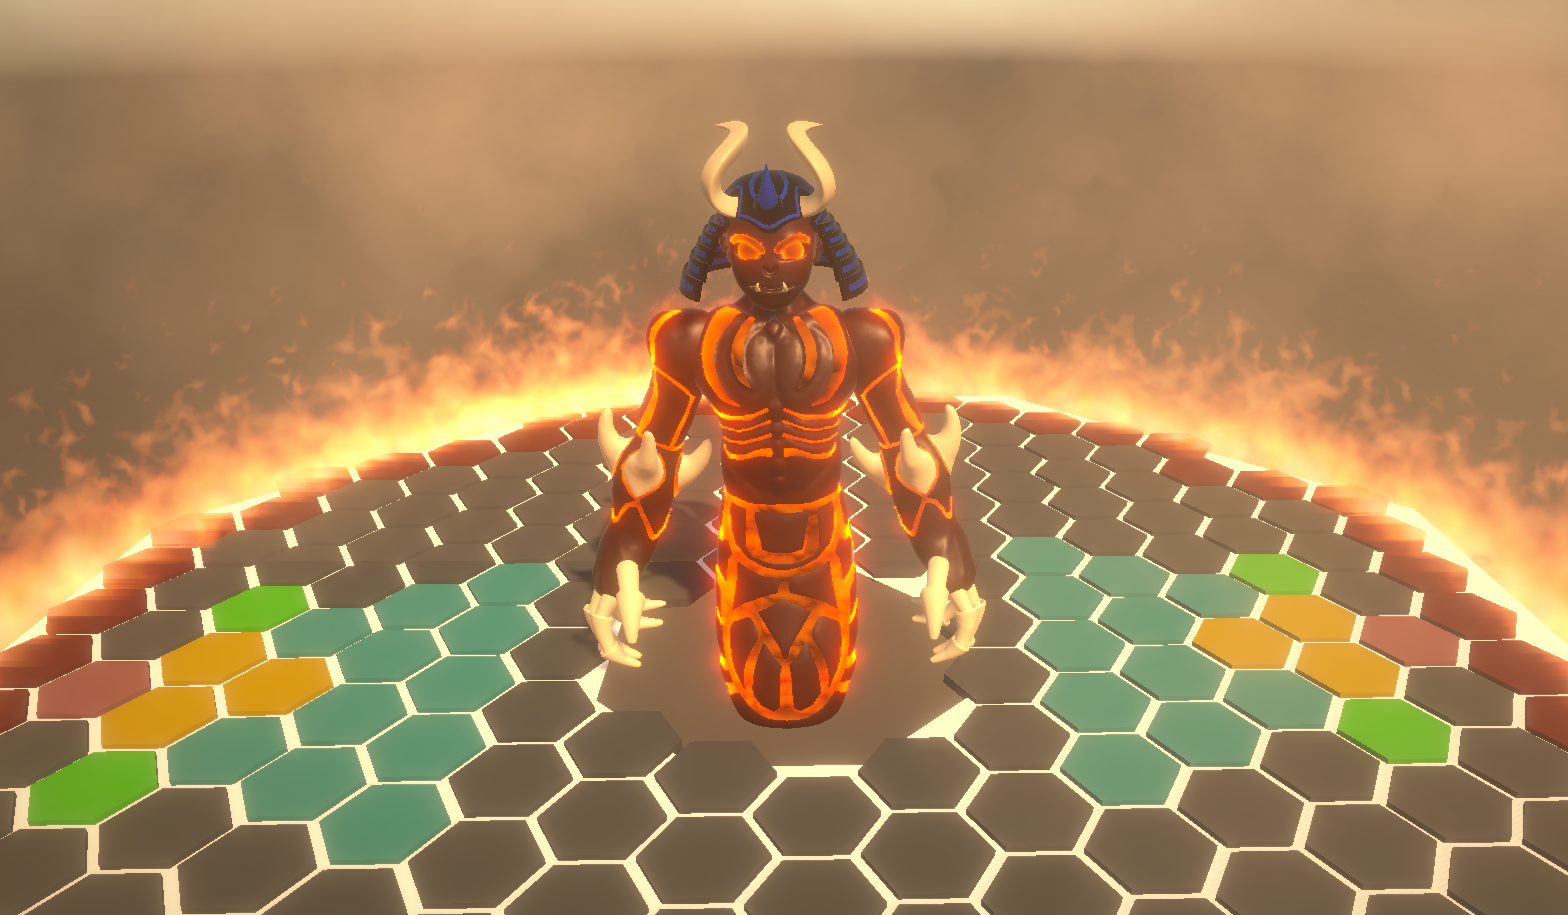
\includegraphics[width=1\textwidth]{fireDemon.png}
		\caption{Monstrul de foc}
		\label{fig: fireDemon}
	\end{figure}
	
	La încărcarea scenei de lupta, în mijlocul hărții apare un monstru imens de foc. Scopul nivelului este să învingem monstrul împreună cu coechipierul nostru, înainte ca acesta să ne distrugă baza.
	
	Acest monstru, o dată la un anumit interval de timp alege să execute o acțiune din acțiunile lui deja staibile. Acțiunile posibile ale acestui monstru sunt următoarele:
	
	\begin{enumerate}
		\item Monstrul începe să se întindă. Este o acțiune care ușurează puțin nivelul deoarece nu atacă jucătorul. Acesta doar arată o animație cum se întinde puțin pe hartă și îi permite jucătorului să se refacă după atacurile anterioare sau să atace monstrul cu tot ce are mai puternic.
		\item \textbf{Distrugătorul de turnuri}. Pentru această acțiune, monstrul de foc ridica mâna dreaptă sus și începe să creeze meteoriți de foc. Acești meteoriți cresc în mărime până în punctul în care ajung la o dimensiune cât un turn obișnuit. În acest moment, monstrul de foc alege la întâmplare un turn de pe hartă, trimite meteoritul către acest turn, după care începe să încarce următorul meteorit. În caz că nu găsește nici un turn pe hartă, atunci va ataca direct una din bazele jucătorilor, altfel, atât timp cât există cel puțin un turn pe hartă, nu poate să atace bazele jucătorilor. Numărul de meteoriți folosiți diferă în funcție de dificultatea aleasă: 3 meteoriți în modul ușor, 5 meteoriți pe mediu și 7 meteoriți pe cea mai mare dificultate.
		\item \textbf{Învârtirea mortală}. Monstrul de foc își scoate ghiarele și începe să se învârtă 360 de grade și să lovească toate turnurile de pe hartă, incluzând bazele jucătorilor. Pentru a diminua daunele primite, jucătorul poate să construiască garduri electrice pentru a proteja toate turnurile din spatele acestora. În caz că monstrul de foc întâlnește garduri electrice, va scădea jumate din viața care ar fi fost scăzută în mod normal. Această diminuare se aplică doar turnurilor care se află fix în spatele gardurilor electrice, cele care se află în lateralul acestora nu primesc acest beneficiu.
		\item \textbf{Meteoritul suprem}. Acest atac nu poate fi ales în mod voit de către monstrul de foc. Este activat automat când monstrul de foc ajunge la 2/3 și 1/3 din viața lui maximă. Pentru acest atac, alege la întâmplare una din bazele jucătorilor, se învârte către această și începe să încarce un meteorit uriaș deasupra capului. Pe ecran apare un cronometru, iar jucătorii au timp 30 de secunde că să îi provoace suficiente daune monstrului. În caz că nu reușesc acest lucru, monstrul va lansa meteoritul uriaș (care este cât un sfert din hartă în punctul acesta) către baza jucătorului, lovind toate turnurile din cale. În cazul în care jucătorii reușesc să îl atace suficient de mult în acest timp, monstrul devine amețit timp de 10 secunde, timp în care jucătorii pot să îl atace sau să își refacă turnurile după bunul plac.
	\end{enumerate}
	
	Pe lângă aceste atacuri, monstrul are și o abilitate automată: cu cât îi scade mai mult viața, cu atât devine mai puternic. Când este aproape de punctul de a muri, va fi de 1.5 ori mai puternic decât era la începutul nivelului.
	\newline
	
	Acest monstru are anumite proprietăți definite într-un fișier configurabil, care a permis crearea cu ușurință a dificultăților multiple. Acest fișier configurabil reprezintă o clasa de tipul BossScriptableObject, care moștenește clasa ScriptableObject. Această clasa definește următoarele proprietăți: viața maximă, timpul dintre decizii, banii primiți de jucător pentru fiecare punct de viață luat, puterea de atac pentru fiecare dintre cele trei atacuri ( distrugătorul de turnuri, învârtirea mortală, meteoritul suprem ), numărul de meteoriți pentru atacul "distrugătorul de turnuri" și procentajul de viață necesar pentru a deveni amețit în momentul când execută atacul "meteoritul suprem".
	\newline
	
	Datorită acestei structuri, am definit 3 fișiere configurabile, câte unul pentru fiecare dificultate și am adăugat opțiunea de a permite jucătorului să aleagă pe care dintre ele le dorește la începerea jocului. Dificultatea poate fi modificată doar de jucătorul care deține camera, dar și celălalt jucător poate să vadă care dificultate este aleasă.
	
	
	
	
	
	\subsection{Metode de îmbunătățire a proiectului}
	
	Jocul a ajuns într-un punct destul de bun, în care poate să fie jucat cap coadă de jucători, iar modul co-op este complet funcțional, dar care este mai mult un exemplu de ce poate devenii. Jocul poate fi îmbunătățit într-o serie de moduri pe care, din nefericire, nu mai am timp să le implementez, dar pe care doresc totuși să le enumerez în acest capitol.
	
	
	
	
	
	\subsubsection{Artă îmbunătățită}
	
	În primul rând, arta este un factor major pentru care oamenii aleg să joace un joc. Arta actuală a jocului este mai mult conceptuală, nu este finisată deloc. Am încercat să definesc câteva turnuri finisate în Blender, dar pentru a crește calitatea jocului trebuie realizate o serie de lucruri legate de aspectul grafic al jocului:
	
	\begin{enumerate}
		\item Toate turnurile să fie schimbate cu modele și materiale realiste pe ele. Pe lângă asta, ar fi util să aibă și animații de construire a turnurilor, distrugere a acestora, și după caz, al atacului.
		\item Hărțile de joc trebuie să fie făcute modele 3D adevărate, ci nu doar niște planșe care definesc zonele pe unde pot să circule inamicii. Aceste nivele ar trebuii ideal să fie environmenturi cu o tonă de alte modele de umplutură. Câteva exemple de hărți realiste ar fi: o hartă pe dealuri, înconjurați de copaci, tufe și alte obiecte/creaturi găsite în natură. În centrul hărții ar fi o zona defroșată unde poți construii turnurile. O altă idee ar fi un oraș abandonat, cu o tematică a culorilor foarte sumbră. Clădirile din oraș pot să construiască un fel de labirint artificial, iar turnurile să poată fi construite pe clădiri, sau între aceste clădiri.
		\item Fiecare nivel sau fiecare hartă să aibă o tematică a culorilor folosite. La început să fie culori deschise și ușoare pentru ochi, iar pe final culorile să devină foarte intense.
		\item Hexagonale pot fi ascunse, și să apară doar în momentul în care dorim să construim un turn. Modul în care apar ar fi folosit un shader transparent, poate chiar cel construit deja.
		\item Efectele speciale pot fi îmbunătățite, și pot fi adăugate efecte speciale pentru acțiunile care nu au fost acoperite încă (îmbunătățirea turnurilor, distrugerea acestora)
		\item Animații la toate UI-urile și tranzițiile între scene.
	\end{enumerate}
	
	\begin{figure}[H]
		\centering
		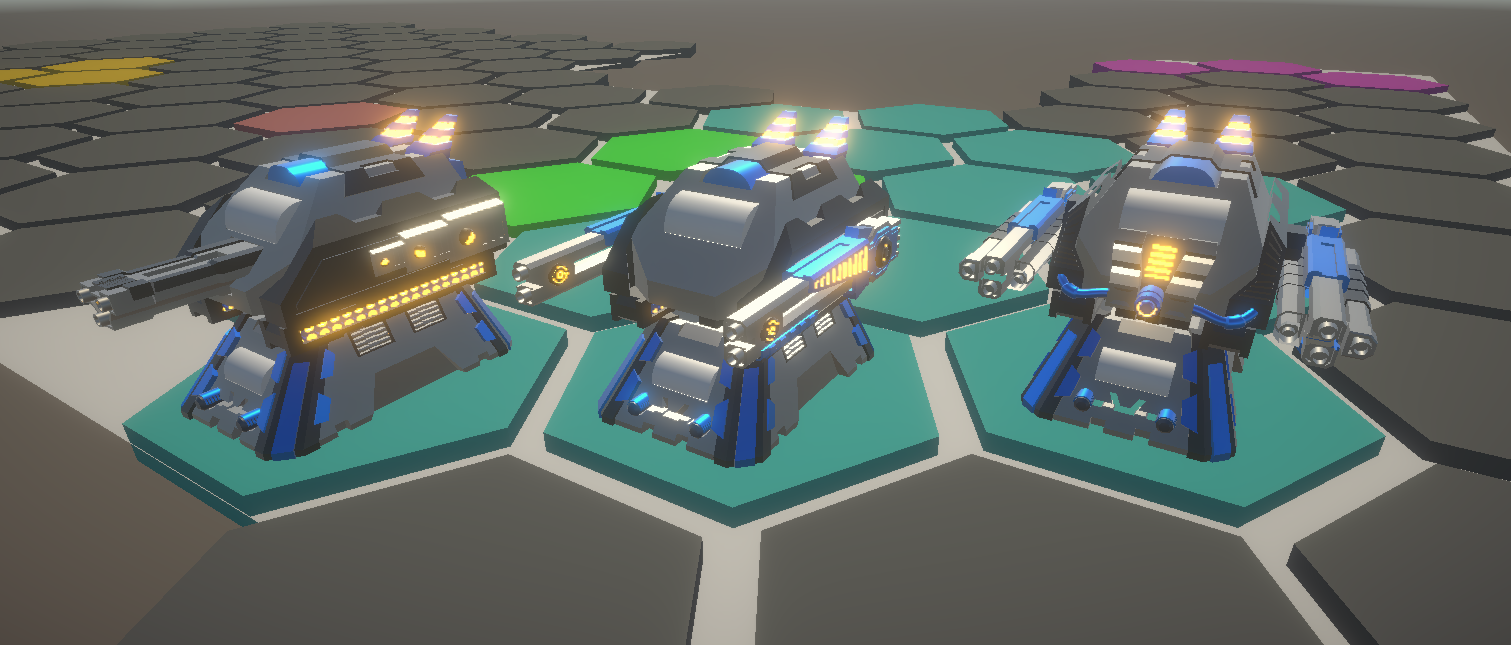
\includegraphics[width=1\textwidth]{betterMachineGun.png}
		\caption{Exemplu de grafică îmbunătățită pentru un turn defensiv}
		\label{fig: betterTurret}
	\end{figure}
	
	
	
	\subsubsection{O poveste pentru joc}
	
	Am definit deja o poveste de bază pentru joc în capitolul \ref{section: gamePlot}, dar aceasta a rămas drept un concept neimplementat. Ar îmbunătății enorm calitatea jocului dacă ar avea o poveste care să descrie evenimentele care au loc. Pe lângă asta, ar fi de dorit un sistem de dialog în care comandantul discuta cu soldații lui, cu centrul de operații de pe planeta mamă sau cu inamicii. Pentru toate aceste interactiuni de dialog, ar putea fi desenate imagini cu caracterele jocului sau s-ar putea folosi direct modelele lor 3D, la care ar trebuii realizate animații faciale, sincronizarea buzelor, și animații specifice în funcție de evenimentele întâmplate (când sunt fericiți, au pierdut o misiune, sunt surprinși, etc.)
	
	
	
	
	\subsubsection{Sunetele pentru joc}
	
	Desigur, nu există joc fără sunete, oricât de retro ar putea să fie jocul. Jocul ar trebuii să aibă câteva melodii de fundal care să acapareze jucătorul. Ideal fiecare harta diferită ar avea o melodie diferită, dar acest lucru ar fi greu de realizat fără o persoană dedicată pe această parte. Sunete de atac și pentru efectele speciale ar fi și ele foarte de dorit, iar la finalul unui nivel ar putea fi adăugate sunete comice în cazul pierderii nivelului.
	
	
	
	
	
	\subsubsection{Monștrii multipli pentru modul co-op}
	
	Inițial am venit cu mai multe concepte pentru monștrii care pot fi adăugați în modul co-op, dar am avut timp să implementez doar unul din aceștia, motiv pentru care o să îi înșirui pe restul aici:
	
	\begin{enumerate}
		\item \textbf{Necromancer}. Este un monstru mai mic decât monstrul de foc și se poate teleporta la diverse locații pe hartă. Are 3 atacuri: un atac în care alege o direcție și lansează o bară oblică care lovește tot ce îi stă în cale, un atac în care cheamă alți inamici pe hartă, inamici care vor ataca toate turnurile pe care le găsesc în cale. Atacul lui special este să se teleporteze în spatele unei baze și să provoace foarte multe daune.
		\item \textbf{Monstrul corosiv}. În fiecare secundă de joc, toate turnurile vor primii daune mici, dar care se adună cu timpul. De asemenea are 3 atacuri: un atac în care scuipă acid într-o zona largă peste turnuri și crește viteza cu care le scade viața. Atacul lui special ar fi că își poate separa corpul în mai multe bile mai mici, care se mișcă încet una spre alta. Dacă acestea se adună toate, mostrul revine la normal și își reface multă viață. Scopul jucătorilor este să distrugă cât mai multe astfel de bile în timpul alocat.
		\item \textbf{Armadillo}. Asemănător vietății cu același nume, este un monstru imens care are foarte multă viață. Din când în când alege să se facă în formă de bilă și să se rostogolească peste toate turnurile de pe harta. Scopul, la fel că și la monstrul de foc, este să îi provoace suficiente daune într-un timp cât mai scurt pentru a îl întrerupe din a ataca. Celelalte atacuri nu au fost definite încă.
	\end{enumerate}
	
	
	
	\subsubsection{Balansarea dificultății}
	
	Desigur, pentru un joc reușit, proprietățile trebuie să fie balansate într-un mod cât mai ideal. Jocul nu trebuie să fie nici foate dificil dar nici extrem de ușor. Jucătorul ar trebuii să se simtă nevoit să conceapă strategii de plasare a turnurilor pentru a reușii să câștige nivelele, iar din când în când să fie nevoit să joace nivelele anterioare și să obțină 3 stele la fiecare, pentru a își îmbunătății turnurile.
	\newline
	
	Balansarea dificultății este o problema serioasă în industria jocurilor, motiv pentru care există persoane specializate care se ocupă de acest lucru și sunt mulți testeri care parcurg jocul și își dau cu părerea despre modul în care poate fi îmbunătățit.
	
	
	
	
	
	\section{Concluzii}
	
	Jocurile video au început să acapareze din ce în ce mai mult viețile noastre, iar industria aceasta este în continuă dezvoltare, motiv pentru care este o arie care merită explorată din perspectiva unui programator și nu numai.
	\newline
	
	Acest proiect a fost realizat în Unity pentru a mari viteza de dezvoltare și a crește calitatea jocului rezultat. În plus, a fost necesară folosirea unor tehnologii specifice în Unity, precum: Photon Network, Shader Graph, VFX Graph, etc.
	\newline
	
	Dezvoltarea proiectului a necesitat o planificare cât mai organizată a functionalitatilor și a modului de implementare, fapt care a ușurat exponențial procesul de dezvoltare. Pe parcursul acestui proiect am documentat o serie de concepte utile de organizare a codului și a modului de lucru din industria profesionistă.
	\newline
	
	Jocul rezultat conține o multitudine de sisteme complexe care interacționează între ele pentru a crea experiențe cât mai interesante pentru utilizatori. Implementarea acestor sisteme a presupus utilizarea multor tehnologii ingenioase, iar rezultatul final este pe măsură așteptărilor.
	\newline
	
	Implementarea experienței co-op a presupus o provocare datorită dificultății de sincronizarea a datelor jucătorilor. Serverul folosit de aplicație este un server oferit gratuit de Photon Engine, iar sincronizarea datelor s-a realizat cu ajutorul functionalitatilor definite de acesta. În ciuda faptului că sincronizarea tuturor obiectelor și interacțiunilor din scenă a presupus o dificultate pentru acest proiect, în cele din urmă a fost realizată cu succes.
	\newline
	
	Acest joc poate să fie îmbunătățit și extins într-o serie de moduri: prin adăugarea unei grafici îmbunătățite, adăugarea sunetelor și melodiilor pentru joc, adăugarea unei povești și a unui sistem de dialog, inamici multiplii pentru modul co-op și prin balansearea corespunzătoare a dificultății.
	\newline
	
	Proiectul a fost distractiv de conceput și recomand tuturor persoanelor care sunt interesate să învețe modul în care funcționează jocurile video, să încerce pe cont propriu un proiect similar cu acesta.
	
	
	
	\pagebreak
	\begin{thebibliography}{3}
		\bibitem{gameProgrammingComplete} 
		Mike McShaffry, David Graham. \newline
		\textit{Game Coding Complete Fourth Edition}. 2012
		
		\bibitem{bookOfLenses}
		Jesse Schell.  \newline
		\textit{The Art of Game Design: A Book of Lenses 1st Edition}. 2008
		
		\bibitem{grafuriAnul2}
		Eleonor Ciurea, Laura Ciupala.  \newline
		\textit{Algoritmi: Introducere în algoritmică fluxurilor în rețele}. 2006
		
		\bibitem{unityAPI}
		https://docs.unity3d.com/ScriptReference/
		
		\bibitem{photonAPI}
		https://doc.photonengine.com/en-us/pun/current/getting-started/pun-intro
		
	\end{thebibliography}
	
	
\end{document}